%!Cau!%
\begin{ex}%[KSCL, Sở GD và ĐT - Thanh Hóa, 2018]%[Bùi Ngọc Diệp, 12EX-5]%[1D2K5-2]
	Xếp ngẫu nhiên $8$ chữ cái trong cụm từ "THANH HOA" thành một hàng ngang. Tính xác suất để có ít nhất hai chữ cái H đứng cạnh nhau
	\choice
	{ $\dfrac{5}{14}$}
	{ $\dfrac{5}{84}$}
	{\True $\dfrac{9}{14}$}
	{ $\dfrac{79}{84}$}
	\loigiai{
		Số phần tử của không gian mẫu là $n(\Omega) = \dfrac{8!}{2! 3!} = 3360$. \\
		Gọi $A$ là biến cố đã cho, ta sẽ tìm số phần tử của $ \overline{A} $. \\
		Đầu tiên ta xếp $2$ chữ cái $A$ và $3$ chữ cái $T, O, N$ có $\dfrac{5!}{2!} = 60$ cách xếp. \\
		Tiếp theo ta có $6$ vị trí (xen  giữa và ở hai đầu) để xếp $3$ chữ cái $H$, có $\mathrm{C}_6^3$ cách xếp. \\
		Do đó $n(\overline{A}) = 60 \cdot \mathrm{C}_6^3 = 1200$, suy ra $n(A) = n(\Omega) - n(\overline{A}) = 3360 - 1200 = 2160$. \\Vậy xác suất cần tìm là $P(A) = \dfrac{n(A)}{n(\Omega)} = \dfrac{2160}{3360} = \dfrac{9}{14}$.}
\end{ex}%!Cau!%
\begin{ex}%[De tap huan, So GD&DT Dien Bien, 2019]%[Ngoc Diep, dự án EX5]%[1D2K5-5]
	Có hai hộp: Hộp I đựng $4$ gói quà màu đỏ và $6$ gói quà màu xanh, hộp II đựng $2$ gói quà màu đỏ và $8$ gói quà màu xanh. Gieo một con súc sắc, nếu được mặt $6$ chấm thì lấy một gói quà từ hộp I, nếu được mặt khác thì lấy một gói quà từ hộp II. Tính xác suất để lấy được gói quà màu đỏ.
	\choice
	{$\dfrac{23}{30}$}
	{$\dfrac{2}{3}$}
	{\True $\dfrac{7}{30}$}
	{$\dfrac{1}{3}$}
	\loigiai{
		Xác suất lấy được gói quà màu đỏ trong hộp $1$ là $\mathrm{P}(A_1) = \dfrac{4}{10} = \dfrac{2}{5}$.\\
		Xác suất lấy được gói quà màu đỏ trong hộp $2$ là $\mathrm{P}(A_2) = \dfrac{2}{10} = \dfrac{1}{5}$.\\
		Xác suất gieo được mặt sáu chấm là $\mathrm{P}(C) = \dfrac{1}{6} $, gieo được một trong $5$ mặt còn lại là $\mathrm{P} \left(  \overline{C} \right)  = \dfrac{5}{6}$.\\
		Do đó xác suất lấy được gói quà màu đỏ là
		$$\dfrac{1}{6} \cdot \dfrac{2}{5} + \dfrac{5}{6} \cdot \dfrac{1}{5} = \dfrac{7}{30}.$$
	}
\end{ex}%!Cau!%
\begin{ex}%[DTH, Sở GD và ĐT - Hà Nam, 2019]%[Đào-V- Thủy, 12EX5]%[1D2K5-2]
	Cho tập $X=\left\{6; 7; 8; 9\right\}$, gọi $E$ là tập các số tự nhiên khác nhau có $2018$ chữ số lập từ các chữ số của tập $X$. Chọn ngẫu nhiên một số trong tập $E$, tính xác suất để chọn được số chia hết cho $3$.
	\choice
	{\True $\dfrac{1}{3}\left(1+\dfrac{1}{2^{4035}}\right)$}
	{$\dfrac{1}{3}\left(1+\dfrac{1}{2^{2017}}\right)$}
	{$\dfrac{1}{3}\left(1+\dfrac{1}{2^{4036}}\right)$}
	{$\dfrac{1}{3}\left(1+\dfrac{1}{2^{2018}}\right)$}
	\loigiai
	{Gọi $A_n$, $B_n$ là tập con của $E$ gồm các số có $n$ chữ số với $A_n$ là tập các số chia hết cho $3$ và $B_n$ là tập các số không chia hết cho $3$.\\
		Với mỗi số thuộc $A_n$ có hai cách thêm vào cuối một chữ số $6$ hoặc $9$ để được $A_{n+1}$ và hai cách thêm vào cuối chữ số $7$ hoặc chữ số $8$ để được $B_{n+1}$.\\
		Với mỗi số thuộc $B_n$ có một cách thêm vào cuối một chữ số $7$ hoặc chữ số $8$ để được $A_{n+1}$ và có ba cách thêm một số để được $B_{n+1}$.\\
		Như vậy $\heva{&|A_{n+1}|=2|A_n|+|B_n|\\&|B_{n+1}|=2|A_n|+3|B_n|}\Rightarrow |B_{n+1}|=3|A_{n+1}|-4|B_n|\Rightarrow |A_{n+1}|=5|A_n|-4|A_{n-1}|$.\\
		Hay $|A_n|=5|A_{n-1}|-4|A_{n-2}|$.\\
		Xét dãy $a_n=|A_n|$, ta có $a_1=2$, $a_2=6$, $a_n=5a_{n-1}-4a_{n-2}$ với $n\geq 3$.\\
		Nên $a_n=\alpha+\beta \cdot 4^n=\dfrac{2}{3}+\dfrac{1}{3}\cdot 4^n$. Suy ra, có $\dfrac{4^{2018}+2}{3}$ số chia hết cho $3$.\\
		Mà $|E|=4^{2018}$.\\
		Vậy xác suất cần tìm là $P=\dfrac{1}{3}\cdot \left(1+\dfrac{1}{2^{4035}}\right)$.
		
	}
\end{ex}%!Cau!%
\begin{ex}%[Thi thử lần I, Sở GD&ĐT Sơn La 2019]%[Nguyễn Anh Quốc,  dự án EX5]%[1D2K5-2]
	Trong một lớp học gồm $15$ học sinh nam và $10$ học sinh nữ. Giáo viên gọi ngẫu nhiên $4$ học sinh lên bảng giải bài tập. Xác suất để $4$ học sinh được gọi có cả nam lẫn nữ là
	\choice
	{\True $\dfrac{443}{506}$}
	{$\dfrac{442}{506}$}
	{$\dfrac{218}{323}$}
	{$\dfrac{219}{323}$}
	\loigiai{Gọi $\Omega$ là không gian mẫu.\\
		Số phần tử không gian mẫu là ${n(\Omega)}=\mathrm{C}_{25}^4$.\\
		Gọi $A\colon$\lq\lq Chọn $4$ học sinh có cả nam lẫn nữ\rq\rq.\\
		Suy ra biến cố $\overline{A}$ là \lq\lq$4$ học sinh được chọn hoặc là nam, hoặc là nữ\rq\rq.\\
		Do đó $n(\overline{A})=\mathrm{C}_{15}^4+\mathrm{C}_{10}^4$.\\
		Khi đó xác suất của biến cố $A$ là  $\mathrm{P}(A)=1-\mathrm{P}(\overline{A})=1-\dfrac{n(\overline{A})}{n(\Omega)}=1-\dfrac{\mathrm{C}_{15}^4+\mathrm{C}_{10}^4}{\mathrm{C}_{25}^4}=\dfrac{443}{506}$.
	}
\end{ex}%!Cau!%
\begin{ex}%[Đề tập huấn, Sở GD - ĐT tỉnh Quảng Bình, 2019]%[Nguyễn Tiến, dự án 12EX5]%[1D2K5-2]
	Một lô hàng có $20$ sản phẩm, trong đó có $4$ phế phẩm. Lấy tùy ý $6$ sản phẩm từ lô hàng đó. Hãy tính xác suất để trong $6$ sản phẩm lấy ra có không quá $1$ phế phẩm.
	\choice
	{$\dfrac{7}{9}$}
	{$\dfrac{91}{323}$}
	{\True $\dfrac{637}{969}$}
	{$\dfrac{91}{285}$}
	\loigiai{
		Lấy $6$ sản phẩm từ $20$ sản phẩm trong lô hàng có $\mathrm{C}_{20}^6=38760$ cách $\Rightarrow n(\Omega)=38760$.\\
		Gọi $X$ là biến cố $6$ sản phẩm lấy ra có không quá $1$ phế phẩm.\\
		Khi đó ta xét các trường hợp sau:\\
		\textbf{TH1:} $6$ sản phẩm lấy ra không có phế phẩm nào $\Rightarrow$ có $\mathrm{C}_{16}^6=8008$ cách.\\
		\textbf{TH2:} $6$ sản phẩm lấy ra có $1$ phế phẩm $\Rightarrow$ có $\mathrm{C}_{16}^5\cdot\mathrm{C}_{4}^1=17472$ cách.\\
		Suy ra số kết quả thuận lợi cho biến cố $X$ là $n(X)=8008+17472=25480$.\\
		Vậy xác suất cần tính là $P=\dfrac{n(X)}{n(\Omega)}=\dfrac{25480}{38760}=\dfrac{637}{969}$.
	}
\end{ex}%!Cau!%
\begin{ex}%[Tập huấn, Sở GD và ĐT lần 1, 2019]%[Lê Xuân Hòa, 12EX5]% [1D2K5-5]
Cho đa giác đều $20$ đỉnh. Trong các tứ giác có $4$ đỉnh là đỉnh của đa giác, chọn ngẫu nhiên một tứ giác. Xác suất để tứ giác được chọn là hình chữ nhật bằng
\choice
{$\dfrac{6}{323}$}
{\True $\dfrac{3}{323}$}
{$\dfrac{15}{323}$}
{$\dfrac{14}{323}$}
\loigiai{
Số tứ giác tạo thành từ $4$ đỉnh trong $20$ đỉnh của đa giác là $\left|\Omega\right|=\mathrm{C}_{20}^4=4845$.\\
Gọi $A$ là biến cố chọn được một tứ giác là hình chữ nhật.\\
Kết quả thuận lợi của biến cố $A$ là $\left|\Omega (A)\right| = \mathrm{C}_{10}^2=45$.\\
Xác suất của biến cố $A$ là $\mathrm{P}(A) = \dfrac{\left|\Omega (A)\right|}{\left|\Omega\right|}=\dfrac{45}{4845}=\dfrac{3}{323}$.
}
\end{ex}%!Cau!%
\begin{ex}%[Tập huấn, Sở GD và ĐT lần 1, 2019]%[Lê Xuân Hòa, 12EX5]%[1D2K5-5]
Gọi $S$ là tập hợp các số tự nhiên nhỏ hơn $10^6$ được lập thành từ hai số $0$ và $1$. Lấy ngẫu nhiên hai số trong $S$. Xác suất để lấy được ít nhất một số chia hết cho $3$ bằng
\choice
{$\dfrac{4473}{8128}$}
{$\dfrac{2279}{4064}$}
{\True $\dfrac{55}{96}$}
{ $\dfrac{53}{96}$}
\loigiai{
Có $a_i \ne 0$; $a_1,\ldots ,a_2\in \left\{ 0,1\right\}$.\\
Số phần tử của $S$ là $2+1\cdot 2 +1\cdot 2\cdot 2 +1\cdot 2\cdot 2\cdot 2 +1\cdot 2\cdot 2\cdot 2\cdot 2 +1\cdot 2\cdot 2\cdot 2\cdot 2\cdot 2 =64$.\\
Lấy ngẫu nhiên hai trong số $S$, có $\mathrm{C}_{64}^2$.\\
Gọi $A$ là biến cố lấy được ít nhất một số chia hết cho $3$.\\
Suy ra $\bar{A}$ là biến cố không lấy được số chia hết cho $3$.\\
Ta xét xem trong $64$ số trong tập $S$ có bao nhiêu số chia hết cho $3$
\begin{enumerate}[TH1]
\item Số có $1$ chữ số $a_1$: có $2$ số và có một số chia hết cho $3$ đó là số $0$.
\item Số có $2$ chữ số $\overline{a_1a_2}$: có $2$ số và cả $2$ số không chia hết cho $3$.
\item Số có $3$ chữ số $\overline{a_1a_2a_3}$: có $4$ số và trong đó có $1$ số chia hết cho $3$.
\item Số có $4$ chữ số $\overline{a_1a_2a_3a_4}$: có $8$ số và trong đó có $3$ số chia hết cho $3$.
\item Số có $4$ chữ số $\overline{a_1a_2a_3a_4a_5}$: có $16$ số và trong đó có $6$ số chia hết cho $3$.
\item Số có $4$ chữ số $\overline{a_1a_2a_3a_4a_5a_6}$: có $32$ số và trong đó có $11$ số chia hết cho $3$.
\end{enumerate}
Do đó,  trong tập $S$ có $22$ số chia hết cho $3$ và có $42$ số không chia hết cho $3$.\\
Khi đó $\mathrm{P}\left(\bar{A}\right) =\dfrac{\mathrm{C}_{42}^2}{\mathrm{C}_{64}^2}=\dfrac{41}{96}$.\\
Vậy $\mathrm{P}(A) = 1- \mathrm{P}\left(\bar{A}\right) =\dfrac{55}{96}$.
}
\end{ex}%!Cau!%
\begin{ex}%[Thi thử, Chuyên Sơn La, 2018]%[Nguyễn Thanh Tâm, 12-EX-5-2019]%[1D2K5-2]
	Cho $(H)$ là đa giác đều $2n$ đỉnh nội tiếp đường tròn tâm $O$ ($n\in {\mathbb{N}}^{*},n\ge 2$). Gọi $S$ là tập hợp các tam giác có ba đỉnh là các đỉnh của đa giác $(H)$. Chọn ngẫu nhiên một tam giác thuộc $S$, biết rằng xác suất chọn được một tam giác vuông trong tập $S$ là $\dfrac{3}{29}$. Tìm $n$. 
	\choice
	{$20$}
	{$12$}
	{\True $15$}
	{$10$}
	\loigiai
	{
		Gọi $A$ là biến cố “chọn được một tam giác vuông”.\\
		Số phần tử của không gian mẫu: $n(\Omega)=\mathrm {C}_{2n}^3$.\\
		Để lập một tam giác vuông như ycđb đầu tiên ta chọn một đường chéo xuyên tâm của đa giác, có $n$ đường chéo như thế nên có $n$ cách chọn; sau đó chọn tiếp $1$ đỉnh của đa giác trong các đỉnh còn lại, có $2n-2$ cách chọn.\\
		Số phần tử thuận lợi cho biến cố: $n(A)=n.(2n-2)$.\\
		Xác xuất của biến cố $A$ bằng $P(A)=\dfrac{n(A)}{n(\Omega)}=\dfrac{n(2n-2)}{\mathrm {C}_{2n}^3}$.\\
		Theo đề ra:
		\begin{eqnarray*}
			& & P(A)=\dfrac{3}{29}\\
			&\Leftrightarrow & \dfrac{n(2n-2)}{\mathrm {C}_{2n}^3}=\dfrac{3}{29}\\
			&\Leftrightarrow & \dfrac{n(2n-2)}{2n(2n-1)(2n-2):3!}=\dfrac{3}{29}\\
			&\Leftrightarrow & 6(2n-1)=29.3!\\
			&\Leftrightarrow & n=15.
		\end{eqnarray*}
		Với đề bài trắc nghiệm có thể giải pt tìm $n$ bằng cách sử dụng mode $7$ với $n$ chạy từ $2$ đến $21$, step $1$.
	}
\end{ex}%!Cau!%
\begin{ex}%[Đề tập huấn, Sở GD và ĐT - Quảng Trị, 2018]%[Nguyễn Văn Nay, 12EX10]%[1D2K5-2]
	Một tổ có $10$ học sinh trong đó có $4$ nam và $6$ nữ. Thầy chủ nhiệm cần chọn một nhóm $3$ học sinh làm trực nhật. Tính xác suất để trong ba người được chọn phải có học sinh nam.
	\choice
	{$\dfrac 16$}
	{$\dfrac 23$}
	{$\dfrac 13$}
	{\True $\dfrac 56$}
	\loigiai{
		Gọi $A$ là biến cố ``trong ba người được chọn có học sinh nam''.\\
		Suy ra biến cố đối $\overline{A}$ ``trong ba người được chọn không có học sinh nam'' 
		hay $\overline{A}$ ``ba người được chọn đều là nữ''.\\
		Xác suất $P(\overline{A})=\dfrac{\mathrm{C}_6^3}{\mathrm{C}_{10}^3}=\dfrac{1}{6}$, do đó $P(A)=1-P(\overline{A})=\dfrac{5}{6}$.
	}
\end{ex}%!Cau!%
\begin{ex}%[Thi tập huấn, Sở GD và ĐT - Bắc Ninh, 2019]%[Nguyễn Minh Tiến, 12EX5]%[1D2K5-5]
	Cho đa giác đều $20$ đỉnh. Trong các tứ giác có bốn đỉnh là đỉnh của đa giác, chọn ngẫu nhiên một tứ giác. Xác suất để tứ giác được chọn là hình chữ nhật là
	\choice
	{$\dfrac{6}{323}$}
	{\True $\dfrac{3}{323}$}
	{$\dfrac{15}{323}$ }
	{$\dfrac{14}{323}$}
	\loigiai{
		Số tứ giác có bốn đỉnh là đỉnh của đa giác là $\mathrm{C}_{20}^4$.\\
		Đa giác đều $20$ đỉnh có $10$ đường chéo qua tâm, cứ hai đường chéo qua tâm cho ta một hình chữ nhật. Vậy số cách chọn ra $4$ đỉnh tạo thành một hình chữ nhật là $\mathrm{C}_{10}^2$.
$\mathrm{P}=\dfrac{\mathrm{C}_{10}^2}{\mathrm{C}_{20}^4}=\dfrac{3}{323}$.
	}
\end{ex}%!Cau!%
\begin{ex}%[Thi tập huấn, Sở GD và ĐT - Bắc Ninh, 2019]%[Nguyễn Minh Tiến, 12EX5]%[1D2K5-5]
	Gọi $S$ là tập hợp các số tự nhiên nhỏ hơn $10^6$ được thành lập từ hai chữ số $0$ và $1$. Lấy ngẫu nhiên hai số trong $S$. Xác suất để lấy được ít nhất một số chia hết cho $3$ là
	\choice
	{$\dfrac{4473}{8128}$}
	{$\dfrac{2279}{4046}$}
	{$\dfrac{55}{96}$ }
	{\True $\dfrac{53}{96}$}
	\loigiai{
		Gọi số có 6 chữ số có dạng $\overline{a_1a_2a_3a_4a_5a_6}$ có: $a_1\ne 0;a_1,\ldots ,a_6\in\{0;1\}$.\\
 Số phần tử của tập $S$ là: $2+1\cdot2+1\cdot 2\cdot 2+1\cdot 2\cdot 2\cdot 2+1\cdot 2\cdot 2\cdot 2\cdot 2 +1\cdot 2\cdot 2\cdot 2\cdot 2=64$.
		\newline Lấy ngẫu nhiên hai số trong $S$ số cách lấy là $\mathrm{C}_{63}^2$.
		\newline Gọi $A$ là biến cố lấy được ít nhất một số chia hết cho $3$.
		\newline $\Rightarrow\overline{A}$ là biến cố không lấy được số chia hết cho $3$.
		\newline Ta xét xem trong $63$ số của tập $S$ có bao nhiêu số chia hết cho $3$.
		\newline +TH1: Số có $1$ chữ số $a_1$: có 2 số và hai số này đều không chia hết cho $3$.
		\newline +TH2: Số có $2$ chữ số $\overline{a_1a_2}$ với $a_1=1:$ có $2$ số và $2$ số này đều chia hết cho $3$.
		\newline +TH3: Số có $3$ chữ số $\overline{a_1a_2a_3}$ với $a_1=1:$ có $4$ số và trong đó có $1$ số chia hết cho $3$.
		\newline +TH4: Số có $4$ chữ số $\overline{a_1a_2a_3a_4}$ với $a_1=1:$ có $8$ số và trong đó có $3$ số chia hết cho $3$.
			\newline +TH5: Số có $5$ chữ số $\overline{a_1a_2a_3a_4a_5}$ với $a_1=1:$ có $16$ số và trong đó có $6$ số chia hết cho $3$.
					\newline +TH6: Số có $6$ chữ số $\overline{a_1a_2a_3a_4a_5a_6}$ với $a_1=1:$ có $32$ số và trong đó có $11$ số chia hết cho $3$.
					\newline Do đó có $21$ số chia được cho $3$ và có $43$ số không chia được cho $3$.
					\newline Do đó $\mathrm{P}(\overline{A}) = \dfrac{\mathrm{C}_{43}^2}{\mathrm{C}_{64}^2} = \dfrac{43}{96}$. Vậy $\mathrm{P}(A) = 1 - \mathrm{P}(\overline{A}) = \dfrac{53}{96}$.
	}
\end{ex}%!Cau!%
\begin{ex}%[Thi thử, Lào Cai - Phú Thọ, 2019]%[Bùi Anh Tuấn, dự án (12EX-5)]%[1D2K5-2]
	Có $ 20 $ tấm thẻ được đánh số từ $ 1 $ đến $ 20 $. Chọn ngẫu nhiên $ 8 $ tấm, tính xác suất để chọn được $ 5 $ tấm mang số lẻ, $ 3 $ tấm mang số chẵn trong đó có ít nhất $ 2 $ tấm mang số chia hết cho $ 4 $, kết quả gần đúng là
	\choice
	{\True $12\%$}
	{$23\%$}
	{$3\%$}
	{ $2\%$}
	\loigiai{ Trong $ 20 $ tấm thẻ có $ 10 $ tấm mang số lẻ, $ 10 $ tấm mang số chẵn và $ 5 $ tấm chia hết cho $ 4 $.\\
		Số phần tử của không gian mẫu là $ \left|\Omega\right|=\mathrm{C}_{20}^8$.\\
		Gọi $ A $ là biến cố chọn được $ 8 $ thẻ thỏa mãn yêu cầu đề bài. Số cách chọn $ 8 $ thẻ trong đó có $ 5 $ thẻ mang số lẻ, $ 3 $ thẻ mang số chẵn trong đó có ít nhất $ 2 $ thẻ mang số chia hết cho $ 4 $ có hai trường hợp xảy ra
		\begin{itemize}
			\item Trường hợp số thẻ chia hết cho $ 4 $ là $ 2 $.\\
			Ta có số cách là $\mathrm{C}_{10}^5\cdot\mathrm{C}_{5}^2\cdot\mathrm{C}_{5}^1$.
			\item Trường hợp số thẻ chia hết cho $ 4 $ là $ 3 $.\\
			Ta có số cách là $\mathrm{C}_{10}^5\cdot\mathrm{C}_5^3$.
		\end{itemize} Suy ra các trường hợp thuận lợi cho biến cố $ A $ là $\left|\Omega_{A}\right|=\mathrm{C}_{10}^5\cdot\mathrm{C}_{5}^2\cdot\mathrm{C}_{5}^1+\mathrm{C}_{10}^5\cdot\mathrm{C}_5^3$.\\
		Vậy xác suất cần tìm là $ \mathrm{P}(A)=\dfrac{\left|\Omega_{A}\right|}{\left|\Omega\right|}=\dfrac{\mathrm{C}_{10}^5\cdot\mathrm{C}_{5}^2\cdot\mathrm{C}_{5}^1+\mathrm{C}_{10}^5\cdot\mathrm{C}_5^3}{\mathrm{C}_{20}^8}=\dfrac{504}{4199}\approx 0{,12}=12\%$.
	}
\end{ex}%!Cau!%
\begin{ex}%[Đề tập huấn, Bắc Kạn, 2018-2019]%[Cao Thành Thái, 12EX5-2019]%[1D2K5-2]
 Trong mặt phẳng với hệ toạ độ $Oxy$, chọn ngẫu nhiên một điểm mà toạ độ của nó là các số nguyên có giá trị tuyệt đối nhỏ hơn hoặc bằng $4$. Nếu các điểm đều có cùng xác suất được chọn như nhau, vậy thì xác suất để chọn được một điểm mà khoảng cách đến gốc toạ độ nhỏ hơn hoặc bằng $2$ là
 \choice
  {\True $\dfrac{13}{81}$}
  {$\dfrac{15}{81}$}
  {$\dfrac{13}{32}$}
  {$\dfrac{11}{16}$}
 \loigiai
  {
  Gọi $M(a; b)$ thuộc mặt phẳng $(Oxy)$. Từ giả thiết ta có $|a|\leq 4$ và $|b|\leq 4$.\\
  Vì $a$, $b$ là số nguyên nên $a$, $b$ thuộc tập $\{-4; -3; -2; -1; 0; 1; 2; 3; 4\}$.\\
  Do đó có $9 \cdot 9=81$ cách chọn một điểm $M(a; b)$ theo yêu cầu.\\
  Giả sử khoảng cách từ điểm $A(x; y)$ đến gốc $O$ nhỏ hơn hoặc bằng $2$, tức là ta có 
  \[x^2+y^2 \leq 4, \tag{$*$}\] với $x$, $y$ là số nguyên.\\
  Ta tìm được $13$ điểm $(x;y)$ thỏa mãn $(*)$ là $(0;0)$, $(0;1)$, $(0;2)$, $(0;-1)$, $(0;-2)$, $(1;0)$, $(2;0)$, $(-1;0)$, $(-2;0)$, $(1;1)$, $(1;-1)$, $(-1;1)$, $(-1;-1)$.\\
  Vì thế xác suất cần tìm là $\dfrac{13}{81}$.
  }
\end{ex}%!Cau!%
\begin{ex}%[Tập huấn SGD Bắc Ninh, Dự án 12EX5, 2019, Chu Đức Minh]%[1D2K5-5]
	Gọi $S$ là tập hợp các số tự nhiên nhỏ hơn $10^6$ được lập thành từ các chữ số $0$ và $1$. Lấy ngẫu nhiên $2$ số trong $S$. Xác suất để lấy được ít nhất một số chia hết cho  $3$ bằng 
	\choice
	{$\dfrac{4473}{8128}$}
	{$\dfrac{2279}{4064}$}
	{$\dfrac{55}{96}$}
	{\True $\dfrac{53}{96}$}
	\loigiai{
		$\bullet$ Tập $S$ gồm các phần tử có dạng $\overline{a_1a_2a_3a_4a_5a_6}$ với $a_i \in \{0;1\}$. Số phần tử của tập $S$ là $2^6=64$ (phần tử). Do đó có $\mathrm{C}^2_{64}$ cách chọn $2$ phần tử trong $S$. \\
		$\bullet$ Số được chọn chia hết cho $3$ khi có đúng $3$ số $1$ hoặc có đúng $6$ số $1$. Do đó có $1 + \mathrm{C}^3_6 = 21$ số chia hết cho $3$ trong tập $S$. Suy ra có $43$ số không chia hết cho $3$ trong $S$. \\
		$\bullet$ Xác suất để chọn được $2$ số không chia hết cho $3$ là $P(\overline{A}) = \dfrac{\mathrm{C}^2_{43}}{\mathrm{C}^2_{64}} = \dfrac{43}{96}$. \\
		$\bullet$ Vậy xác suất để chọn được ít nhất $1$ số chia hết cho $3$ là $\dfrac{53}{96}$. 
	}
\end{ex}%!Cau!%
\begin{ex}%[Thi thử, Sở GD và ĐT - Hà Tĩnh, 2019]%[Đặng Tân Hoài, 12-EX-5-2019]%[1D2K5-2]
	Rút ngẫu nhiên cùng lúc $2$ chiếc bút từ một hộp chứa $4$ bút chì và $5$ bút bi. Xác suất để $2$ bút rút được đều là bút chì bằng
	\choice
	{$\dfrac{1}{2}$}
	{\True $\dfrac{1}{6}$}
	{$\dfrac{2}{9}$}
	{$\dfrac{5}{18}$}
	\loigiai{
	Số phần tử của không gian mẫu là $n(\Omega)=\mathrm{C}_9^2$.\\
	Gọi $A$ là biến cố \lq \lq rút được $2$ bút đều là bút chì \rq \rq \,. Khi đó $n(A)=\mathrm{C}_4^2$.\\
	Vậy xác suất cần tính là $P(A)=\dfrac{n(A)}{n(\Omega)}=\dfrac{1}{6}$.
	}
\end{ex}%!Cau!%
\begin{ex}%[Thi thử lần 2, THPT Nguyễn Đức Cảnh, 2019]%[Nguyễn Anh Tuấn, 12EX7]%[1D2K5-2]
	Cho một đa giác đều có $ 20 $ đỉnh nội tiếp trong một đường tròn $ (C) $. Lấy ngẫu nhiên hai đường chéo trong số các đường chéo của đa giác. Tính xác suất để lấy được hai đường chéo cắt nhau và giao điểm của hai đường chéo này nằm bên trong đường tròn.
	\choice
	{$ \dfrac{17}{63} $}
	{\True $ \dfrac{57}{169} $}
	{$ \dfrac{19}{63} $}
	{$ \dfrac{19}{169} $}
	\loigiai{
	Số đường chéo của đa giác đều $ 20 $ đỉnh là $ \mathrm{C}_{20}^2-20=170 $.\\
	Xét phép thử lấy ngẫu nhiên hai đường chéo trong số các đường chéo của đa giác, suy ra số phần tử của không gian mẫu là $ n(\Omega)=\mathrm{C}_{170}^2=14365 $.\\
	Gọi $ A $ là biến cố: "Lấy được hai đường chéo cắt nhau và giao điểm của hai đường chéo này nằm bên trong đường tròn". \\
	Nhận xét: Mỗi tứ giác nội tiếp đường tròn $ (C) $, có duy nhất hai đường chéo cắt nhau và giao điểm của chúng nằm trong đường tròn, do đó $ n(A)=\mathrm{C}_{20}^4 =4845$.\\
	Vậy $ \mathrm{P}(A)=\dfrac{4845}{14365}= \dfrac{57}{169}$.
	}
\end{ex}%!Cau!%
\begin{ex}%[Đề thi thử Chuyên Sơn La lần 1, Sơn La, 2018-2019]%[Cao Thành Thái, dự án 12-EX-7-2019]%[1D2K5-2]
 Gọi $S$ là tập hợp các số tự nhiên có chín chữ số đôi một khác nhau. Chọn ngẫu nhiên một số thuộc tập $S$. Xác suất để số được chọn chia hết cho $3$ bằng
 \choice
  {\True $\dfrac{11}{27}$}
  {$\dfrac{21}{32}$}
  {$\dfrac{12}{27}$}
  {$\dfrac{23}{32}$}
 \loigiai
  {
  Trước hết ta tính $n(S)$. Với số tự nhiên có chín chữ số đôi một khác nhau thì chữ số đầu tiên có $9$ cách chọn và có $\mathrm{A}_9^8$ cách chọn cho tám vị trí còn lại. Vậy $n(S)=9\mathrm{A}_9^8$.\\
  Giả sử $B=\{0;1;2;\ldots;9\}$, ta thấy tổng các phần tử của $B$ bằng $45\ \vdots\ 3$ nên số có chín chữ số đôi một khác nhau và chia hết cho $3$ sẽ được tạo thành từ $9$ chữ số của các tập $B\setminus\{0\}$, $B\setminus\{3\}$, $B\setminus\{6\}$, $B\setminus\{9\}$, suy ra số các số loại này là $\mathrm{A}_9^9+3\cdot 8\cdot \mathrm{A}_8^8$.\\
  Vậy xác suất cần tìm là $\dfrac{\mathrm{A}_9^9+3\cdot 8\cdot \mathrm{A}_8^8}{9\mathrm{A}_9^8} = \dfrac{11}{27}$.
  }
\end{ex}%!Cau!%
\begin{ex}%[Dự án EX-7-2019]%[Phạm Tuấn]%[1D2K5-2]
Gọi $A$ là tập hợp tất cả các số tự nhiên gồm $4$ chữ số phân biệt được chọn từ các chữ số
$0;1; 2;3;4;5;6$. Chọn ngẫu nhiên một số từ tập $A$, tính xác suất để số chọn được là số chia hết cho $5$
và lớn hơn $2000$.
\choice
{$\dfrac{5}{18}$}
{$\dfrac{11}{36}$}
{\True $\dfrac{1}{4}$}
{$\dfrac{2}{9}$}
\loigiai{
Giả sử $\overline{abcd} \in A$. Có $6$ cách chọn $a$, $\mathrm{A}_6^3$ cách chọn cách chọn và sắp xếp các chữ số còn lại. Suy ra $|A|= 6\mathrm{A}_6^3 = 720 \Rightarrow n(\Omega) = 720$.  \\
Nếu $\overline{abcd} \in A$, $\overline{abcd}~\vdots~ 5$ và $\overline{abcd} >2000$ thì $a \geqslant 2$ và $d=0$ hoặc $d=5$. 
\begin{itemize}
\item Với $d=0$: có $5$ cách chọn $a$, $\mathrm{A}_5^2$ cách  chọn và sắp xếp hai chữ số  $b,c$. Vậy có $5 \mathrm{A}_5^2$ số thỏa mãn. 
\item Với $d=5$: có $4$ cách chọn $a$, $\mathrm{A}_5^2$ cách  chọn và sắp xếp hai chữ số  $b,c$. Vậy có $4 \mathrm{A}_5^2$ số thỏa mãn. 
\end{itemize}
Xác suất để số chọn được là số chia hết cho $5$ và lớn hơn $2000$ bằng
\[ 
\dfrac{5\mathrm{A}_5^2+4\mathrm{A}_5^2}{720} = \dfrac{1}{4}.
\]
}
\end{ex}%!Cau!%
\begin{ex}%[Thi thử L1, THPT Ngô Quyền - Hà Nội, 2019]%[Phan Ngọc Toàn, dự án EX7]%[1D2K5-2]
	Cho $ A $ là tập tất cả các số tự nhiên có $ 5 $ chữ số. Chọn ngẫu nhiên một số từ tập $ A $, tính xác suất để chọn được một số chia hết cho $ 7 $ và chữ số hàng đơn vị là chữ số  $ 1 $.
	\choice
	{\True $\dfrac{643}{45000} $}
	{$ \dfrac{1285}{90000} $}
	{$ \dfrac{107}{7500} $}
	{$ \dfrac{143}{10000} $}
	\loigiai{
		Gọi $ A $ là biến cố ``Chọn được một số chia hết cho $ 7 $ và chữ số hàng đơn vị là chữ số  $ 1 $''.\\
		Ta có số các số tự nhiên có $ 5 $ chữ số là $ 9 \cdot 10^4 = 90000$, suy ra $ n (\Omega ) = 90000$.\\
		Gọi số tự nhiên có $ 5 $ chữ số, chia hết cho $ 7 $ và chữ số hàng đơn vị là chữ số  $ 1 $ là $ x= \overline{abcd1} $.\\
		Ta có $ x = \overline{abcd1} = 10 \overline{abcd} + 1 = \left( 3 \overline{abcd} + 1\right)  + 7 \overline{abcd} $. Do đó $ x $ chia hết cho $ 7 $ khi $ 3 \overline{abcd} + 1 $ chia hết cho $ 7 $, nghĩa là 
		\begin{eqnarray*}
			& &3 \overline {abcd} + 1 = 7k,\ k \in \mathbb{N}\\
			&\Leftrightarrow & \overline{abcd} = 2k + \dfrac{k - 1}{3} ,\ k \in \mathbb{N} \\
			&\Leftrightarrow & \overline{abcd} = 7t + 2,\  t = \dfrac{k - 1}{3},\ t \in \mathbb{N} \\
			&\Rightarrow & 1000 \le 7t + 2 \le 9999 ,\ t \in \mathbb{N} \\
			&\Leftrightarrow & \dfrac{998}{7} \le t \le \dfrac{9997}{7},\ t \in \mathbb{N} \\
			&\Leftrightarrow & \ t \in \{ 143; 144; \ldots ; 1428 \}.
		\end{eqnarray*}
		Suy ra $ n(A) = 1286  \Rightarrow \mathrm{P}(A) = \dfrac{1286}{90000} = \dfrac{643}{45000} $. 		
	}
\end{ex}%!Cau!%
\begin{ex}%[Thi thử L2, THPT Nguyễn Trung Thiên - Hà Tĩnh, 2019]%[Nguyễn Thành Nhân,12EX7]%[1D2K5-2]
Đoàn trường THPT Nguyễn Đình Liễn tổ chức giao lưu bóng chuyền học sinh giữa các lớp nhân dịp chào mừng ngày 26/03. Sau quá trình đăng ký có $10$ đội tham gia thi đấu từ $10$ lớp, trong đó có $10$ A1 và $10$ A2, các đội chia làm hai bảng, ký hiệu là bảng $A$ và bảng $B$, mỗi bảng $5$ đội. Việc chia bảng được thực hiện bằng cách bốc thăm ngẫu nhiên. Tính xác xuất để hai đội $10$ A1 và $10$ A2 thuộc hai bảng đấu khác nhau.     
	\choice
	{ \True $\dfrac{5}{9}$  }
	{$\dfrac{5}{18}$ }
	{$\dfrac{10}{18}$ }
	{$\dfrac{9}{10}$}
	\loigiai{ Gọi $A$ là biến cố \lq\lq Hai đội $10$ A1 và $10$ A2 ở hai bảng khác nhau \rq\rq \\
	Số cách xếp $10$ đội vào hai bảng khác nhau là $n\left( \Omega \right)=\mathrm{C}_{10}^5 \cdot \mathrm{C}_5^5= 252$.\\
	Số cách để $10$ A1 chọn bảng là $ \mathrm{C}_2^1$.\\
	Số cách để $10$ A2 chọn bảng là $\mathrm{C}_1^1$.\\
	Số cách xếp $8$ đội còn lại vào hai bảng là                   $\mathrm{C}_8^4 \cdot \mathrm{C}_4^4$.\\
	Vậy $\mathrm{n}(A)= 2\cdot 1\cdot 70=140$.\\
	Vậy xác suất của biến cố $A$ là $\mathrm{P}(A)=\dfrac{140}{252}=\dfrac{5}{9}$. 
	 }
\end{ex}%!Cau!%
\begin{ex}%[Thi thử, THPT Chuyên Ngoại Ngữ - Hà Nội, 2019]%[Trần Nhân Kiệt, 12EX7-2019]%[1D2K5-5]
Một hộp kín chứa $50$ quả bóng kích thước bằng nhau, được đánh số tử $1$ đến $50$. Bốc ngẫu nhiên
cùng lúc $2$ quả bóng từ hộp trên. Gọi $\mathrm{P}$ là xác suất bốc được $2$ quả bóng có tích của $2$ số ghi trên $2$ quả bóng là một số chia hết cho $10$, khẳng định nào sau đây đúng?
	\choice
	{$0{,}2<\mathrm{P}<0{,}25$}
	{$0{,}3<\mathrm{P}<0{,}35$}
	{\True $0{,}25<\mathrm{P}<0{,}3$}
	{$0{,}35<\mathrm{P}<0{,}4$}
	\loigiai{
Số cách chọn ngẫu nhiên $2$ quả bóng trong hộp là $n(\Omega)=\mathrm{C}_{50}^2=1225$ cách chọn.\\
Gọi $A$ là biến cố \lq\lq chọn được $2$ quả bóng có tích của $2$ số ghi trên $2$ quả bóng là một số chia hết cho $10$ \rq\rq.
\begin{itemize}
\item[TH1.] Chọn được một quả bóng chia hết cho $10\Rightarrow$ có $5$ cách chọn.\\
Quả bóng còn lại có $45$ cách chọn.\\
$\Rightarrow$ có $5\cdot 45=225$ cách chọn.
\item[TH2.] Chọn được một quả bóng ghi số chẵn nhưng tận cùng không phải là chữ số $0\Rightarrow$ có $20$ cách chọn.\\
Quả bóng còn lại có số ghi trên quả bóng phải có tận cùng là $5\Rightarrow$ có $5$ cách chọn.\\
$\Rightarrow$ có $20\cdot 5=100$ cách chọn.\\
Do đó $n(A)=225+100=335$. 
\end{itemize}
Xác suất cần tìm là $\mathrm{P}(A)=\dfrac{n(A)}{n(\Omega)}=\dfrac{325}{1225}=\dfrac{13}{49}\approx 0{,}27$.

	}
\end{ex}%!Cau!%
\begin{ex}%[Thi thử, trường THPT Nguyễn Công Trứ, tỉnh Hà Tĩnh, 2019]%[Phạm Doãn Lê Bình, 12EX7-19]%[1D2K5-5]
	Một đề kiểm tra Toán Giải tích chương $2$ của khối $11$  có $20$  câu trắc nghiệm. Mỗi câu có  $4$ phương án lựa chọn, trong đó chỉ có  $1$ đáp án đúng. Một học sinh không học bài nên đánh hú họa câu trả lời. Tính xác suất để học sinh đó nhận được  $6$ điểm (kết quả làm tròn đến $4$ chữ số sau dấu phẩy thập phân).
	\choice
	{$0{,}7873$}
	{$\dfrac{1}{4}$}
	{$0{,}0609$}
	{\True $0{,}0008$}
	\loigiai{
	Mỗi phương án trả lời đúng sẽ ứng với $0{,}5$ điểm.\\
	Để học sinh nhận được $6$ điểm thì học sinh đó phải đánh đúng đáp án của $12$ câu và sai $8$ còn lại. Do có $20$ câu nên số trường hợp đúng $12$ trong số $20$ câu là $\mathrm{C}_{20}^{12}$.\\ 	
	Xác suất để đánh trúng trong một câu là $\dfrac{1}{4}$ và đánh sai là $\dfrac{3}{4}$. \\
	Xác suất để học sinh đó được $6$ điểm là  $\mathrm{C}_{20}^{12} \cdot \left( \dfrac{1}{4} \right)^{12} \cdot \left( \dfrac{3}{4} \right)^8 \approx 0{,}0008$.
	}
\end{ex}%!Cau!%
\begin{ex}%[Thi thử, Toán học tuổi trẻ, 2019-2]%[Nguyễn Trường Sơn, 12-EX-5-2019]%[1D2K5-4]
	Gieo một con súc sắc năm lần liên tiếp. Xác suất để tích các số chấm xuất hiện ở năm lần giao đó là một số tự nhiên có tận cùng bằng $5$ là
	\choice
	{$\dfrac{1}{2}$}
	{\True $\dfrac{211}{7776}$}
	{$\dfrac{2}{3}$}
	{$\dfrac{5}{486}$}
	\loigiai{
		Gọi  $\Omega$ là không gian mẫu, $A$ là biến cố “gieo một con súc sắc năm lần liên tiếp có tích các số chấm xuất hiện ở năm lần gieo là một số tự nhiên có tận cùng bằng  $5$”.\\
		Gieo súc sắc năm lần liên tiếp nên $n(\Omega)=6^5$.\\
		Để tích các số chấm xuất hiện ở năm lần gieo là một số tự nhiên có tận cùng bằng  $5$ thì các mặt xuất hiện phải có số chấm lẻ và xuất hiện mặt $5$ chấm ít nhất một lần nên  $n(A)=3^5-2^5=221$.\\
		Suy ra:  $\mathrm{P}(A)=\dfrac{221}{7776}$.	}
\end{ex}%!Cau!%
\begin{ex}%[Thi thử, Toán học tuổi trẻ, 2019-2]%[Nguyễn Trường Sơn, 12-EX-5-2019]%[1D2K5-3]
	Một túi đựng $20 $ tấm thẻ được đánh số từ $1$ tới $20$. Rút ngẫu nhiên ra hai tấm thẻ. Xác suất để tích của hai số ghi trên hai tấm thẻ rút được là một số chia hết cho $4$ bằng
	\choice
	{$\dfrac{1}{3}$}
	{\True $\dfrac{1}{2}$}
	{$\dfrac{1}{4}$}
	{$\dfrac{2}{3}$}
	\loigiai{Số cách chọn ngẫu nhiên ra $2$ tấm thẻ là $\mathrm{C}_{20}^2$.\\
		Gọi $A$ là biến cố:" Rút được hai thẻ có tích của hai số ghi trên hai tấm thẻ rút được là một số chia hết cho $4$".\\ 
		Để tích hai tấm thẻ rút ra chia hết cho $4$, ta có các khả năng:
		\begin{itemize}
			\item Khả năng 1. Chọn được hai thẻ đánh số chẵn, có $\mathrm{C}_{10}^2$ cách.
			\item Khả năng 2. Hai tấm thẻ một thẻ mang số chẵn thuộc tập $\left\lbrace 4,8,12,16,20\right\rbrace $, một thẻ mang số lẻ có $5 \cdot 10=50$ cách. 
		\end{itemize}
	Vậy xác xuất bằng $\mathrm{P}(A)=\dfrac{50+\mathrm{C}_{10}^2}{\mathrm{C}_{20}^2}=\dfrac{1}{2}$.	
	}
\end{ex}%!Cau!%
\begin{ex}%[Thử sức trước kì thi đề số 4, THTT, 2019]%[Trần Hòa, 12EX-7-2019]%[1D2K5-2]
	Gọi $S$ là tập hợp các số tự nhiên có $4$ chữ số lập được từ tập hợp $X=\{1,2,3,4,5,6,7,8,9\}$. Chọn ngẫu nhiên một số từ tập $S$. Tính xác suất để số được chọn là số chia hết cho $6$.
	\choice
	{\True $\dfrac{4}{27}$}
	{$\dfrac{4}{28}$}
	{$\dfrac{9}{25}$}
	{$\dfrac{4}{9}$}
	\loigiai{
	Số các số có $4$ chữ số tạo từ tập $X$ là $9^4=6561.$	\\
	Vậy tập $S$ có $6561$ số.\\
	Gọi số có $4$ chữ số được chọn từ tập $S$ và là số chia hết cho $6$ có dạng $\overline{abcd}$.\\
	Do $\overline{abcd}$ chia hết cho $6$ nên $a+b+c+d$ chia hết cho $3$ và $d$ chẵn $\Rightarrow d\in\{2;4;6;8\}$.\\
	Chọn $b$, $c$ mỗi chữ số có $9$ cách chọn. Ta có $4\cdot9\cdot9=324$ số dạng $\overline{bcd}$.\\
	Xét mỗi số trong số $324$ số dạng  $\overline{bcd}$
	\begin{itemize}
        \item Nếu $b+c+d=3k$ thì $a\in \{3;6;9\}\Rightarrow$ có $3$ cách chọn $a$.
        \item Nếu $b+c+d=3k+1$ thì $a\in \{2;5;8\}\Rightarrow$ có $3$ cách chọn $a$.
        \item Nếu $b+c+d=3k+2$ thì $a\in \{1;4;7\}\Rightarrow$ có $3$ cách chọn $a$.
        \end{itemize}
	Như vậy mỗi số trong số $324$ số dạng  $\overline{bcd}$ có $3$ cách chọn $a$, suy ra có $324\cdot 3=972$ số.\\
	Xác suất cần tính là $\mathrm{P}=\dfrac{972}{6561}=\dfrac{4}{27}.$
	}
\end{ex}%!Cau!%
\begin{ex}%[Thi thử L1, Chuyên Lương Thế Vinh Đồng Nai, 2019]%[Nguyễn Tất Thu, dự án(12EX-7)]%[1D2K5-2]
	Nhằm chào mừng ngày thành lập Đoàn TNCS Hồ Chí Minh, Đoàn trường THPT chuyên Lương Thế Vinh đã tổ chức giải bóng đá nam. Có $16$ đội đăng kí tham dự, trong đó có $3$ đội $10$ Toán, $11$ Toán và $12$ Toán. Ban tổ chức cho bốc thăm ngẫu nhiên để chia đều $16$ đội vào $4$ bảng để đá vòng loại. Tính xác suất để $3$ đội của $3$ lớp Toán nằm ở $3$ bảng khác nhau.
	\choice
	{$ \dfrac{53}{56} $}
	{$ \dfrac{19}{28} $}
	{\True $ \dfrac{16}{35}$}
	{$ \dfrac{3}{56} $}
	\loigiai{ 
	Ta có $n(\Omega)=\mathrm{C}_{16}^4\cdot \mathrm{C}_{12}^4\cdot \mathrm{C}_{8}^4\cdot \mathrm{C}_{4}^4.$\\
Chọn $3$ trong $4$ bảng đấu có $\mathrm{C}_4^3$ cách chọn. Chọn $1$ trong $3$ lớp Toán có $\mathrm{C}_3^1$. Chọn $3$ đội trong $13$ đội còn lại không có đội Toán có $\mathrm{C}_{13}^3$ . Chọn $1$ trong $2$ lớp Toán có $\mathrm{C}_2^1$. Chọn $3$ đội trong $10$ đội còn lại không có đội Toán có $\mathrm{C}_{10}^3$ . Chọn $3$ đội trong $7$ đội còn lại không có đội Toán có $\mathrm{C}_{7}^3$ . Bốn đội còn lại không có đội Toán ở bảng cuối cùng. Do đó theo quy tắc nhân ta có số kết quả thuận lợi cho biến cố $A$ là $$n\left({A}\right)=\mathrm{C}_4^3\cdot \mathrm{C}_3^1\cdot \mathrm{C}_{13}^3\cdot \mathrm{C}_2^1\cdot \mathrm{C}_{10}^3\cdot \mathrm{C}_{7}^3.$$ 
Do đó xác suất của biến cố $A$ là $$p\left({A}\right)=\dfrac{n\left({A}\right)}{n\left({\Omega }\right)}=\dfrac{\mathrm{C}_4^3\cdot \mathrm{C}_3^1\cdot \mathrm{C}_{13}^3\cdot \mathrm{C}_2^1\cdot \mathrm{C}_{10}^3\cdot \mathrm{C}_{7}^3}{\mathrm{C}_{16}^4\cdot \mathrm{C}_{12}^4\cdot \mathrm{C}_{8}^4}=\dfrac{16}{35} .$$

 }
\end{ex}%!Cau!%
\begin{ex}%[Đề KSCL lớp 12 môn Toán Sở giáo dục và đào tạo Thanh Hóa, 2018-2019]%[Cao Thành Thái, dự án 12-EX-8-2019]%[1D2K5-2]
 Gọi $S$ là tập hợp tất cả các số tự nhiên có bốn chữ số đôi một khác nhau được chọn từ các chữ số $1$, $2$, $3$, $4$, $5$, $6$, $7$, $8$, $9$. Lấy ngẫu nhiên một số thuộc $S$. Tính xác suất để lấy được một số chia hết cho $11$ và tổng bốn chữ số của nó cũng chia hết cho $11$.
 \choice
  {$\mathrm{P} = \dfrac{8}{21}$}
  {$\mathrm{P} = \dfrac{2}{63}$}
  {$\mathrm{P} = \dfrac{1}{126}$}
  {\True $\mathrm{P} = \dfrac{1}{63}$}
 \loigiai
  {
  Số phần tử của $S$ là $n(S) = \mathrm{A}_9^4 = 3024$.\\
  Gọi số tự nhiên cần tìm thuộc $S$ là $\overline{abcd}$.\\
  Ta có $\overline{abcd} = 1000a + 100b + 10c + d = 1001a+ 99b + 11c + (-a-c) + (b+d)$. Do đó $\overline{abcd}\,\vdots\, 11$ khi và chỉ khi $\left[b+d-(a+c)\right]\, \vdots\, 11$.\\
  Theo giả thiết ta có $a+b+c+d \,\vdots\, 11$. Suy ra $(a+c)\, \vdots\, 11$ và $(b+d)\, \vdots\, 11$.\\
  Các cặp có tổng chia hết cho $11$ là $(2;9)$, $(3;8)$, $(4;7)$, $(5;6)$.\\
  Vậy số cách chọn số $\overline{abcd}$ thỏa mãn là $n(A) = 4\cdot 3 \cdot 2! \cdot 2! = 48$.\\
  Do đó xác suất cần tìm là $\mathrm{P} = \dfrac{48}{3024} = \dfrac{1}{63}$.
  }
\end{ex}%!Cau!%
\begin{ex}%[Thi thử, Sở GD và ĐT - BRVT, 2019]%[Phan Văn Thành, 12EX8]%[1D2K5-2]
	Gọi $S$ là tập hợp tất cả các số tự nhiên có $7$ chữ số và chia hết cho $9$. Chọn ngẫu nhiên một số từ tập $S$, tính xác suất để các chữ số của số đó đôi một khác nhau. 
	\choice
	{$ \dfrac{512}{3125} $}
	{\True $ \dfrac{198}{3125} $}
	{$ \dfrac{396}{6250} $}
	{$ \dfrac{369}{6250} $}
	\loigiai{
		Gọi không gian mẫu $\Omega$ là \lq\lq số tự nhiên có $7$ chữ số và chia hết cho $9$\rq\rq. Khi đó $n(\Omega) = 1000000$.\\
		Gọi biến cố $A$ là \lq\lq Các chữ số đôi một khác nhau và chia hết cho $9$\rq\rq.\\
		Từ các chữ số $0; 1; 2; \ldots; 9$ ta có các bộ gồm $7$ số có tổng chia hết cho $9$ là\\
		$\{0; 2; 3; 4; 5; 6; 7\}$; $\{0; 1; 3; 4; 5; 6; 8\}$; $\{0; 1; 2; 4; 5; 7; 8\}$; $\{0; 1; 2; 3; 6; 7; 8\}$; $\{0; 3; 4; 5; 7; 8; 9\}$;\\ $\{0; 2; 4; 6; 7; 8; 9\}$; $\{0; 1; 5; 6; 7; 8; 9\}$; $\{0; 1; 2; 3; 4; 8; 9\}$; $\{0; 1; 2; 3; 5; 7; 9\}$; $\{0; 1; 2; 4; 5; 6; 9\}$;\\ $\{2; 3; 4; 5; 6; 7; 9\}$; $\{1; 3; 4; 5; 6; 8; 9\}$; $\{1; 2; 4; 5; 7; 8; 9\}$; $\{1; 2; 3; 6; 7; 8; 9\}$.\\
		Có $10$ bộ số gồm $7$ số có tổng chia hết cho $9$ trong đó có số $0$ nên từ các bộ số này lập được $10 \cdot 6 \cdot 6! = 43200$ số có $7$ chữ số đôi một khác nhau và chia hết cho $9$.\\
		Có $4$ bộ số gồm $7$ số có tổng chia hết cho $9$ tương tự như bộ số $\{2; 3; 4; 5; 6; 7; 9\}$, nên từ các bộ số này lập được $4 \cdot 7! = 20160$ số có $7$ chữ số đôi một khác nhau và chia hết cho $9$.\\
		Do đó $n(A) = 43200 + 20160 = 63360$.\\
		Vậy xác suất của biến cố $A$ là $\mathrm{P}(A) = \dfrac{n(A)}{n(\Omega)} = \dfrac{63360}{10000000} = \dfrac{198}{3125}$.
	}
\end{ex}%!Cau!%
\begin{ex}%[Thi thử, Sở GD và ĐT - Lào Cai, 2019]%[Lê Thanh Nin, 12EX8]%[1D2K5-2]
	Giải bóng chuyền VTV Cup có $12$ đội bóng tham dự trong đó có $9$ đội nước ngoài và $3$ đội của Việt Nam. Ban tổ chức cho bốc thăm ngẫu nhiên để chia thành $3$ bảng đấu $A$, $B$, $C$ mỗi bảng có $4$ đội. Xác suất để $3$ đội Việt Nam nằm ở $3$ bảng đấu khác nhau bằng
	\choice
	{$\mathrm{P}=\dfrac{\mathrm{C}_9^3\mathrm{C}_6^3}{\mathrm{C}_{12}^4\mathrm{C}_8^4}$}
	{$\mathrm{P}=\dfrac{2\mathrm{C}_9^3\mathrm{C}_6^3}{\mathrm{C}_{12}^4\mathrm{C}_8^4}$}
	{\True $\mathrm{P}=\dfrac{6\mathrm{C}_9^3\mathrm{C}_6^3}{\mathrm{C}_{12}^4\mathrm{C}_8^4}$}
	{$\mathrm{P}=\dfrac{3\mathrm{C}_9^3\mathrm{C}_6^3}{\mathrm{C}_{12}^4\mathrm{C}_8^4}$}
	\loigiai{
	Số phần tử của không gian mẫu là $n\left(\Omega \right)=\mathrm{C}_{12}^4.\mathrm{C}_8^4\cdot\mathrm{C}_4^4=\mathrm{C}_{12}^4\cdot\mathrm{C}_8^4$.\\
	Gọi $D$ là biến cố \lq\lq $3$ đội Việt Nam nằm ở $3$ bảng đấu khác nhau\rq\rq. \\
	Số cách xếp $3$ đội Việt Nam ở $3$ bảng khác nhau là $3!=6$ (cách).\\
	Số cách xếp $9$ đội còn lại vào $3$ bảng trên là $\mathrm{C}_9^3.\mathrm{C}_6^3$. Do đó $n(D)=6.\mathrm{C}_9^3\cdot \mathrm{C}_6^3$.\\
	Vậy $\mathrm{P}=\dfrac{6\mathrm{C}_9^3\mathrm{C}_6^3}{\mathrm{C}_{12}^4\mathrm{C}_8^4}$.}
\end{ex}%!Cau!%
\begin{ex}%[Thi thử, Kinh Môn - Hải Dương, 2019]%[Lê Vũ Hải, 12EX8]%[1D2K5-2]
	Đội tuyển học sinh giỏi tỉnh gồm có $5$ học sinh lớp $12$ và $3$ học sinh lớp $11$. Chọn ngẫu nhiên từ đội tuyển một học sinh, rồi chọn thêm một học sinh nữa. Tình xác suất để lần thứ hai chọn được học sinh lớp $12$.
	\choice
	{$ \dfrac{5}{14} $}
	{$ \dfrac{25}{28} $}
	{$ \dfrac{15}{28} $}
	{\True $ \dfrac{5}{8} $}
	\loigiai{
		Chọn hai học sinh từ đội tuyển có $8\cdot 7 = 56$ cách.\\
		Chọn học sinh thỏa bài toán có $2$ trường hợp xảy ra
		\begin{itemize}
			\item Trường hợp 1: lần đầu chọn trúng học sinh lớp $11$ và lần sau chọn học sinh lớp $12$ có $3\cdot 5 = 15$ cách.
			\item Cả hai lần đều chọn trúng học sinh lớp $12$ có $5\cdot 4=20$ cách.
		\end{itemize}
		Vậy số cách chọn thỏa lần thứ hai chọn được học sinh lớp $12$ là  $15+20=35$. \\
		Suy ra xác suất cần tìm là $\dfrac{35}{56}=\dfrac{5}{8}$.
	}
\end{ex}%!Cau!%
\begin{ex}%[Đề thi thử trường THPT chuyên Sơn La lần 2, 2019]%[Trần Hòa, 12EX-8-2019]%[1D2K5-2]
	Kết quả $(b;c)$ của việc gieo một con súc sắc cân đối và đồng chất hai lần liên tiếp, trong đó $b$ là số chấm xuất hiện ở lần gieo thứ nhất, $c$ là số chấm xuất hiện ở lần gieo thứ hai được thay vào phương trình bậc hai $x^2+bx+c=0$. Xác suất để phương trình bậc hai đó vô nghiệm là
	\choice
	{$\dfrac{7}{12}$}
	{\True $\dfrac{17}{36}$}
	{$\dfrac{23}{36}$}
	{$\dfrac{5}{36}$}
	\loigiai{
	Gieo một con súc sắc hai lần số kết quả là $36$.\\
	Phương trình $x^2+bx+c=0$ có $\Delta =b^2-4c$.\\
	Phương trình vô nghiệm khi $\Delta <0\Leftrightarrow b^2<4c\Leftrightarrow c>\dfrac{b^2}{4}\quad(*)$.\\
	Do $b,c\in\{1;2;3;4;5;6\}$, để thỏa mãn $(*)$ có các trường hợp sau
	\begin{itemize}
        \item TH1: $b=1$, từ $(*)\Rightarrow c>\dfrac{1}{4}$ có $6$ cách chọn $c$.
        \item TH2: $b=2$, từ $(*)\Rightarrow c>1$ có $5$ cách chọn $c$.
        \item TH3: $b=3$, từ $(*)\Rightarrow c>\dfrac{9}{4}$ có $4$ cách chọn $c$.
        \item TH4: $b=4$, từ $(*)\Rightarrow c>4$ có $2$ cách chọn $c$.
        \end{itemize}
	Vậy tất cả có $6+5+4+2=17$ cách chọn thỏa mãn.\\
	Xác suất thỏa mãn yêu cầu bài toán là $\dfrac{17}{36}$.
	
		
	}
\end{ex}%!Cau!%
\begin{ex}%[Chuyên ĐHSPHN - 19]%[Phan Anh - EX8]%[1D2K5-2]
Một hộp đựng $5$ thẻ được đánh số $3$, $5$, $7$, $11$, $13$. Rút ngẫu nhiên $3$ thẻ. Xác suất để 3 số ghi trên $3$ thẻ đó là $3$ cạnh của một tam giác là
\choice
{$\dfrac{1}{4}$}
{$\dfrac{1}{3}$}
{\True $\dfrac{1}{2}$}
{$\dfrac{2}{5}$}
\loigiai{
Xét phép thử ``Rút ngẫu nhiên 3 thẻ từ hộp đựng 5 thẻ'', suy ra $n\left(\Omega\right)=\mathrm{C}_5^3=10$.\\
Gọi $A$ là biến cố ``$3$ số ghi trên $3$ thẻ đó là $3$ cạnh của một tam giác''.\\
Để rút được $3$ thẻ mà $3$ số ghi trên đó là $3$ cạnh của 1 tam giác thì tổng $2$ số bất kì trong $3$ số lớn hơn số còn lại và hiệu $2$ số bất kì trong $3$ số nhỏ hơn số còn lại.\\
Vậy ta chọn được các bộ số là $\{3;5;7\}$, $\{3;11;13\}$, $\{5;7;11\}$, $\{5;11;13\}$, $\{7;11;13\}$.\\
Ta có $n(A)=5\Rightarrow\mathrm{P}(A)=\dfrac{n(A)}{n(\Omega)}=\dfrac{5}{10}=\dfrac{1}{2}$.}
\end{ex}%!Cau!%
\begin{ex}%[Thi thử L2, Chuyên Lê Quý Đôn - Đà Nẵng, 2019]%[Đinh Thanh Hoàng, 12-EX-8-2019]%[1D2K5-2]
	Chọn ngẫu nhiên ba đỉnh bất kì từ các đỉnh của một đa giác đều $12$ cạnh $A_1A_2\ldots A_{12}$. Tính xác suất để ba đỉnh được chọn tạo thành một tam giác cân.
	\choice
	{$\dfrac{13}{55}$}
	{$\dfrac{12}{55}$}
	{\True $\dfrac{3}{11}$}
	{$\dfrac{5}{11}$}
	\loigiai{
		Xét đường kính $A_1A_7$ khi đó có $5$ cặp điểm đối xứng qua $A_1A_7$ là $\left\lbrace A_2;A_{12}\right\rbrace $, $\left\lbrace A_3;A_{11}\right\rbrace $, $\left\lbrace A_4;A_{20}\right\rbrace $, $\left\lbrace A_5;A_9\right\rbrace $, $\left\lbrace A_6;A_8\right\rbrace $. Khi đó, các cặp điểm này tạo với $A_1$ hoặc $A_7$ ta đều được tam giác cân.\\
		Do đó, số tam giác cân là $2\cdot 5\cdot 6=60$.\\
		Xác suất cần tính là: $\mathrm{P}=\dfrac{60}{\mathrm{C}_{12}^3}=\dfrac{3}{11}$.
	}
\end{ex}%!Cau!%
\begin{ex}%[Thi thử L1, THPT Quỳnh Lưu 2, Nghệ An, 2019]%[Nguyễn Quang Tân, dự án 12-EX-8-2019]%[1D2K5-2]
	Một trường THPT có $10$ lớp $12$, mỗi lớp cử $3$ học sinh tham gia vẽ tranh cổ động. Các lớp tiến hành bắt tay giao lưu với nhau (các học sinh cùng lớp không bắt tay với nhau). Tính số lần bắt tay của các học sinh với nhau, biết rằng hai học sinh khác nhau ở hai lớp khác nhau chỉ bắt tay đúng $1$ lần.
	\choice
	{\True $405$}
	{$435$}
	{$432$}
	{$425$}
	\loigiai{Mỗi lớp cử ra $3$ học sinh nên $10$ lớp cử ra $30$ học sinh. \\
		Suy ra số lần bắt tay là $C_{30}^2$ (bao gồm các học sinh cùng lớp bắt tay với nhau). \\
		Số lần bắt tay của các học sinh học cùng một lớp là $10 \cdot C_3^2$. \\
		Vậy số lần bắt tay của các học sinh với nhau thỏa mãn yêu cầu là  $C_{30}^2 - 10 \cdot C_3^2 = 405$. }
\end{ex}%!Cau!%
\begin{ex}%[Thi thử L1, THPT Quỳnh Lưu 2, Nghệ An, 2019]%[Nguyễn Quang Tân, dự án 12-EX-8-2019]%[1D2K5-1]
	\immini
	{
		Trên mặt phẳng $Oxy$, ta xét một hình chữ nhật $ABCD$ với các điểm $A(-2;0)$, $B(-2;2)$, $C(4;2)$, $D(4;0)$ (hình vẽ). Một con châu chấu nhảy trong hình chữ nhật đó tính cả trên cạnh hình chữ nhật sao cho chân nó luôn đáp xuống mặt phẳng tại các điểm có tọa độ nguyên (tức là
		điểm có cả hoành độ và tung độ đều nguyên). Tính xác suất để nó đáp xuống các điểm $M(x;y)$ mà $x+y<2$.
		\choice{$\dfrac{4}{7}$}{\True $\dfrac{3}{7}$}{$\dfrac{1}{3}$}{$\dfrac{8}{21}$}
	}
	{
		\begin{tikzpicture}[>=stealth,line cap=round,line join=round,scale=.8,font=\footnotesize]
		\tkzDefPoints{-2/0/A, -2/2/B, 4/2/C, 4/0/D, 0/2/E, 2/0/I}
		\draw[->] (-3,0)--(0,0) node[below right]{$O$}--(5,0) node[below]{$x$};
		\draw[->] (0,-3) --(0,4) node[right]{$y$};
		\foreach \x in {1}{
			\draw (\x,0) node[below]{$\x$} circle (1pt);
		}
		\foreach \y in {}{
			\draw (0,\y) node[left]{$\y$} circle (1pt);
		}
		\tkzDrawPoints(A,B,C,D,E,I)
		\tkzDrawSegments[dashed](A,B B,C C,D)
		\draw (4,-2)--(-2,4) node [above] {$x+y=2$};
		\tkzLabelPoints[above right](B,E,C)
		\tkzLabelPoints[below](A,I,D)
		\end{tikzpicture}
	}
	\loigiai{
		Số các điểm có tọa độ nguyên thuộc hình chữ nhật là $7\cdot 3=21$ điểm vì $\heva{& x\in \{-2;-1;0;1;2;3;4\} \\ & y\in \{0;1;2\}.}$\\
		Để con châu chấu đáp xuống các điểm $M(x;y)$ có $x+y<2$ thì con châu chấu sẽ nhảy trong
		khu vực hình thang $BEIA$. Để $M(x;y)$ có tọa độ nguyên thì $\heva{& x\in \{-2;-1;0;1;2\} \\ & y\in \{0;1;2\}.}$
		\begin{itemize}
			\item Nếu $x\in \{-2;-1\}$ thì $y\in \{0;1;2\}$. Vậy có $6$ điểm.
			\item Nếu $x=0$ thì $y \in\{0 ; 1\}\Rightarrow 2$ điểm.
			\item Nếu $x=1 \Rightarrow y=0 \Rightarrow$ có $1$ điểm.
		\end{itemize}
		Vậy xác suất cần tìm là $\dfrac{9}{21}=\dfrac{3}{7}$.
	}
\end{ex}%!Cau!%
\begin{ex}%[TT, THPT Kim Liên, Hà Nội-L2]%[Nguyễn Quang Dũng, dự án 12 EX-8-2019]%[1D2K5-1]
Một người muốn gọi điện thoại nhưng nhớ được các chữ số đầu mà quên mất ba chữ số cuối của số cần gọi. Người đó chỉ nhớ rằng ba chữ số cuối đó phân biệt và có tổng bằng $5$. Tính xác suất để người đó bấm máy một lần đúng số cần gọi.
\choice
{$\dfrac{1}{24}$}
{$\dfrac{1}{36}$}
{\True $\dfrac{1}{12}$}
{$\dfrac{1}{60}$}
\loigiai{
Giả sử $3$ chữ số cuối của số điện thoại là $X=\overline{abc}$ mà $a,b,c$.\\
Ta có $a+b+c=5$ và $a,b,c$ khác nhau thì bộ 3 số khác nhau có tổng bằng $5$ là $\{2;0;3\},\{1;0;4\}$.\\
Xét một bộ, mỗi số điện thoại ứng với một hoán vị của $3$ số trên $\Rightarrow$ số phần tử của không gian mẫu là $n(\Omega)=2\times 3! =12$.\\
Xác suất để người đó bấm một lần đúng số cần gọi là $\dfrac{1}{12}$.}
\end{ex}%!Cau!%
\begin{ex}%[Thi thử THPTQG 2019 môn Toán lần 2 trường Nho Quan A – Ninh Bình,2019]%[Nguyễn Thành Nhân,12EX8]%[1D2K5-2]
Một hộp đựng $11$ tấm thẻ đánh số từ $1$ đến $11$. Chọn ngẫu nhiên $6$ tấm thẻ. Gọi $P$ là xác suất để tổng số ghi trên $6$ tấm thẻ là một số lẻ. Khi đó $P$ bằng
	\choice
	{ \True $\dfrac{118}{231}$}
	{    $\dfrac{100}{231}$ }
	{ $\dfrac{115}{231}$  }
	{   $\dfrac{1}{2}$}
	\loigiai{ Số phần tử của không gian mẫu là: $n(\Omega)=\mathrm{C}_{11}^6=462$.\\
	Gọi $A$ là biến cố \lq\lq Tổng các số ghi trên 6 tấm thẻ là một số lẻ \rq\rq.\\
	Ta có $5$ thẻ ghi số chẵn và $6$ thẻ ghi số lẻ.\\
	Để tổng của $6$ số ghi trên $6$ tấm thẻ là một số lẻ thì số các thẻ ghi số lẻ phải là một số lẻ.\\
	Do đó xảy ra các trường hợp số thẻ ghi số lẻ là $1;3;5$ thẻ. \\
	Số kết quả thuận lợi cho biến cố $A$ là
	$$n(A)=\mathrm{C}_{6}^1 \times \mathrm{C}_{5}^5+\mathrm{C}_{6}^3 \times \mathrm{C}_{5}^3+\mathrm{C}_{6}^5 \times \mathrm{C}_{5}^1=236.$$
	Vậy xác xuất của biến cố $A$ là: $P=\dfrac{236}{462} =\dfrac{118}{231}$.
	  }
\end{ex}%!Cau!%
\begin{ex}%[KTCL 12 L4, Ninh Bình - Bạc Liêu, 2018-2019]%[Vũ Nguyễn Hoàng Anh, 12EX8-19]%[1D2K5-2]
	\immini{
		Cho một quân cờ đứng ở vị trí trung tâm của một bàn cờ $9\times 9$ (xem hình vẽ). Biết rằng, mỗi lần di chuyển, quân cờ chỉ di chuyển sang ô có cùng một cạnh với ô đang đứng. Tính xác suất để sau bốn lần di chuyển, quân cờ không trở về đúng vị trí ban đầu.
		\choice
		{\True $\dfrac{55}{64}$}
		{$\dfrac{1}{3}$}
		{$\dfrac{7}{8}$}
		{$\dfrac{3}{8}$}
	}{
		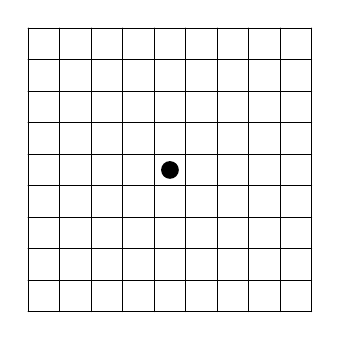
\begin{tikzpicture}[scale=0.4, font=\footnotesize, line join=round, line cap=round]
		\draw (0,0) grid (9,9);
		\fill[black] (4.5,4.5) circle (8pt);
		\end{tikzpicture}
	}
	\loigiai{
		Quân cờ có bốn hướng di chuyển trái, phải, lên, xuống.
		Số cách quân cờ di chuyển tùy ý sau $4$ lần di chuyển là $4^4$.
		Để quân cờ về vị trí ban đầu có $2$ trường hợp.
		\begin{itemize}
			\item Mỗi hướng $1$ lần, có $4!=24$ cách.
			\item Di chuyển $2$ lần lên trên và $2$ lần xuống dưới, hoặc di chuyển $2$ lần sang trái và $2$ lần sang phải, có $2\cdot\dfrac{4!}{2!\cdot 2!}=12$ cách.
		\end{itemize}
		Xác suất cần tìm là $1-\dfrac{24+12}{4^4}= \dfrac{55}{64}$.
	}
\end{ex}%!Cau!%
\begin{ex}%[Thi thử  L2, trường Phúc Trạch-Hà Tĩnh, 2019]%[Lê Hồng Phi, 12EX8]%[1D2K5-2]
Giải bóng chuyền quốc tế VTV Cup có $12$ đội tham gia, trong đó có $3$ đội Việt Nam. Ban tổ chức bốc thăm ngẫu nhiên để chia thành $3$ bảng đấu, mỗi bảng $4$ đội. Tính xác suất để $3$ đội của Việt Nam cùng nằm ở một bảng đấu.
\choice
{$\dfrac{1}{110}$}
{$\dfrac{1}{330}$}
{$\dfrac{6}{55}$}
{\True $\dfrac{3}{55}$}
\loigiai{
Số phần tử của không gian mẫu là $n\left(\Omega\right)=\mathrm{C}_{12}^4\cdot\mathrm{C}_8^4$.\\
Gọi $A$ là biến cố \lq\lq 3 đội của Việt Nam cùng nằm ở một bảng đấu\rq\rq.\\
Chọn ra $3$ đội của Việt Nam và $1$ đội khác rồi xếp chung vào $1$ trong $3$ bảng có $3\cdot\mathrm{C}_9^1$ cách.\\
Chọn ra $4$ đội trong $8$ đội còn lại để được bảng tiếp theo có $\mathrm{C}_8^4$ cách.\\
Bảng còn lại có $1$ cách chọn.\\
Số kết quả thuận lợi cho biến cố $A$ là $n(A)=3\cdot\mathrm{C}_9^1\cdot\mathrm{C}_8^4$.\\
Vậy $\mathrm{P}(A)=\dfrac{3\cdot\mathrm{C}_9^1\cdot\mathrm{C}_8^4}{\mathrm{C}_{12}^4\cdot\mathrm{C}_8^4}=\dfrac{3}{55}$.}
\end{ex}%!Cau!%
\begin{ex}%[thi thử, THPT Triệu Thái, Vĩnh Phúc]%[Phan Quốc Trí, dự án 12EX-8-2019]%[1D2K5-2]
	Trong kỳ thi chọn học sinh giỏi tỉnh có $105$ em dự thi, có $10$ em tham gia buổi gặp mặt trước kỳ thi. Biết các em đó có số thứ tự trong danh sách lập thành một cấp số cộng. Các em ngồi ngẫu nhiên vào hai dãy bàn đối diện nhau, mỗi dãy có $5$ ghế và mỗi ghế chỉ ngồi được $1$ học sinh. Tính xác suất để tổng các số thứ tự của hai em ngồi đối diện nhau là bằng nhau.	
	\choice
	{$\dfrac{1}{954}$}
	{\True $\dfrac{1}{945}$}
	{$\dfrac{1}{126}$}
	{$\dfrac{1}{252}$}
	\loigiai{
		Số phần tử của không gian mẫu là $n\left( \Omega \right) = 10!=3628800$.\\
		Gọi $A$ là biến cố: \lq \lq Tổng các số thứ tự của hai em ngồi đối diện nhau là bằng nhau\rq \rq .\\
		Giả sử số thứ tự của em thứ $i$ là $u_i$, $(i=1\ldots10)$.\\ Vì dãy số   $(u_i)$ là một cấp số cộng có $10$ số hạng nên 
		$$u_1 + u_{10}=u_2 + u_9 = u_3 + u_8=u_4+u_7 =u_5 + u_6.$$
		Ta cần xếp $5$ cặp học sinh như trên vào $5$ cặp ghế đối diện nhau. Trong mỗi cặp học sinh lại có $2!$ cách xếp $2$ học sinh vào $2$ ghế. Do đó $n(A)=5! \cdot (2!)^5 = 3840$.
		$$\Rightarrow \mathrm{P}(A)=\dfrac{n(A)}{n(\Omega)}=\dfrac{3840}{3628800}=\dfrac{1}{945}. $$
	}
\end{ex}%!Cau!%
\begin{ex}%[Thi thử L1, Chuyên Nguyễn Trãi, Hải Dương, 2019]%[Đinh Thanh Hoàng, dự án EX6]%[1D2K5-2]
	Cho tập $S=\left\{1; 2; 3; \ldots; 19; 20\right\}$ gồm $20$ số tự nhiên từ $1$ đến $20$. Lấy ngẫu nhiên ba số thuộc $S$. Xác suất để ba số lấy được lập thành một cấp số cộng là
	\choice
	{$\dfrac{7}{38}$}
	{$\dfrac{5}{38}$}
	{\True $\dfrac{3}{38}$}
	{$\dfrac{1}{114}$}
	\loigiai{
		Lấy $3$ phần tử từ tập $S$ có $\mathrm{C}_{20}^3$ (cách).\\
		Suy ra số phần tử của không gian mẫu là $n(\Omega)=\mathrm{C}_{20}^3=1140$.\\
		Gọi $A$ là biến cố thỏa mãn yêu cầu bài toán.\\
		Đặt $S_1=\left\{1; 3; 5; \ldots; 19\right\}$, tập $S_1$ có $10$ phần tử; $S_2=\left\{2; 4; 6; \ldots; 20\right\}$, tập $S_2$ có $10$ phần tử.\\
		Ta có $a$, $b$, $c$ là ba số theo thứ tự lập thành cấp số cộng $\Leftrightarrow 2a=b+c$.\\
		Có $2a$ là số chẵn, nên $b$ và $c$ cùng chẵn hoặc cùng lẻ.\\
		Suy ra số cách chọn $b$, $c$ là $2\mathrm{C}_{10}^2$.\\
		Mỗi cách chọn cặp $b$, $c$ thì có duy nhất một cách chọn $a$ sao cho $2a=b+c$.\\
		Suy ra số phần tử của biến cố là $n(A)=2\mathrm{C}_{10}^2=90$.\\
		Xác suất thỏa yêu cầu bài là $\mathrm{P}(A)=\dfrac{n(A)}{n(\Omega)}=\dfrac{90}{1140}=\dfrac{3}{38}$.
	}
\end{ex}%!Cau!%
\begin{ex}%[Thi thử L2, Thanh Chương 1 Nghệ An, 2019]%[Nguyễn Văn Nay, dự án EX8]%[1D2K5-2]
	Một nhóm có $8$ học sinh gồm $4$ bạn nam và $4$ bạn nữ, trong đó có $1$ cặp sinh đôi $1$ nam, $1$ nữ. Xếp ngẫu nhiên $8$ học sinh này vào $2$ dãy ghế đối diện, mỗi dãy $4$ ghế, sao cho mỗi ghế có đúng một học sinh ngồi. Xác suất để cặp sinh đôi ngồi cạnh nhau và nam nữ không ngồi đối diện nhau bằng
	\choice
	{$P=\dfrac{3}{70}$}
	{$P=\dfrac{2}{35}$}
	{$P=\dfrac{2}{105}$}
	{\True $P=\dfrac{3}{140}$}
	\loigiai{
		Số phần tử của không gian mẫu là $|\Omega|=8!$.\\
		Gọi biến cố $A$ :``Cặp sinh đôi ngồi cạnh nhau và nam nữ không ngồi đối diện nhau''.\\
		Chọn vị trí cho 1 cặp sinh đôi có $6$ cách.\\
		Số cách xếp cặp sinh đôi ngồi cạnh nhau $6 \cdot 2!$ cách.\\
		Chọn $1$ học sinh nam ngồi đối diện với học sinh nam sinh đôi $3$ cách.\\
		Chọn $1$ học sinh nữ ngồi đối diện với học sinh nữ sinh đôi $3$ cách.\\
		Còn $4$ vị trí, học sinh nam thứ $3$ có $4$ cách chọn.\\
		Học sinh nữ thứ $3$ có $2$ cách chọn.\\
		Vậy $|A|=6\cdot 2! \cdot3\cdot3 \cdot4 \cdot 2$.\\
		Suy ra $P(A)=\dfrac{6\cdot2 ! \cdot3\cdot3 \cdot4 \cdot2}{8 !}=\dfrac{3}{140}$.	
	}
\end{ex}%!Cau!%
\begin{ex}%[Thi thử L2, Sở GD \& ĐT Bắc Ninh, 2019]%[Trần Toàn, dự án EX9]%[1D2K5-2]
	Gọi $A$ là tập các số tự nhiên có $3$ chữ số đôi một khác nhau. Lấy ngẫu nhiên ra từ $A$ hai số. Tính	xác suất để lấy được hai số mà các chữ số có mặt ở hai số đó giống nhau.
	\choice
	{\True $ \dfrac{41}{5823} $}
	{$ \dfrac{35}{5823} $}
	{$ \dfrac{41}{7190} $}
	{$ \dfrac{14}{1941} $}
	\loigiai{
		Ta có số các số tự nhiên có $3$ chữ số đôi một khác nhau là $9\cdot 9\cdot 8= 648$, trong đó có $9\cdot 8\cdot 7= 504$ số không chứa chữ số $0$.\\
		Khi đó $n(\Omega)=\mathrm{C}_{648}^2$.\\
		\textbf{Trường hợp 1:} Xét các số tự nhiên có $3$ chữ số đôi một khác nhau và không chứa chữ số $0$.\\
		Khi đó số cách chọn ra được hai số mà các chữ số có mặt ở hai số đó giống nhau là $\dfrac{\mathrm{C}_{504}^1\cdot \mathrm{C}_5^1}{2}$ (vì mỗi số được kể $2$ lần).\\
		\textbf{Trường hợp 2:} Xét các số tự nhiên có $3$ chữ số đôi một khác nhau và chứa chữ số $0$.\\
		Khi đó số cách chọn ra được hai số mà các chữ số có mặt ở hai số đó giống nhau là $\dfrac{\mathrm{C}_{144}^1\cdot \mathrm{C}_3^1}{2}$.\\
		Vậy xác suất để lấy được hai số mà các chữ số có mặt giống nhau là:
$$\mathrm{P}=\dfrac{\dfrac{\mathrm{C}_{504}^1\cdot \mathrm{C}_5^1}{2} +\dfrac{\mathrm{C}_{144}^1\cdot \mathrm{C}_3^1}{2} }{\mathrm{C}_{648}^2}= \dfrac{41}{5823}.$$
	}
\end{ex}%!Cau!%
\begin{ex}%[Thi Thử, SGD Quảng Bình]%[Trần Bá Huy, dự án EX-9-2019]%[1D2K5-2]
	Tại SEA Games $2019$, môn bóng chuyền nam có $8$ đội bóng tham dự, trong đó có hai đội tuyển Việt Nam và Thái Lan. Các đội bóng được chia ngẫu nhiên thành $2$ bảng có số đội bóng bằng nhau. Xác suất để hai đội Việt Nam và Thái Lan nằm ở $2$ bảng khác nhau bằng
	\choice
	{$\dfrac{3}{7}$}
	{\True $\dfrac{4}{7}$}
	{$\dfrac{3}{14}$}
	{$\dfrac{11}{14}$}
	\loigiai{
		Số phần tử của không gian mẫu bằng số cách chia một cách ngẫu nhiên $8$ đội bóng thành $2$ bảng, suy ra $\mathrm{n}(\Omega)=\dfrac{1}{2}\mathrm{C}_8^4=35$.\\
		Gọi $A$ là biến cố ``Hai đội Việt Nam và Thái Lan nằm ở $2$ bảng khác nhau''. Ta có $$\mathrm{n}(A)=2\cdot\dfrac{1}{2}\mathrm{C}_6^3=20.$$
		Vậy xác suất của biến cố $A$ bằng $\mathrm{P}(A)=\dfrac{\mathrm{n}(A)}{\mathrm{n}(\Omega)}=\dfrac{20}{35}=\dfrac{4}{7}$.
	}
\end{ex}%!Cau!%
\begin{ex}%[Thi thử, Sở GD và ĐT - Bình Thuận, 2019]%[Huỳnh Xuân Tín, 12EX9]%[1D2K5-2] 
	Gọi $S$ là tập hợp tất cả các số tự nhiên gồm $9$ chữ số đôi một khác nhau. Chọn ngẫu nhiên một số từ $S$. Tính xác suất để số được chọn có đúng  $4$ chữ số lẻ và chữ số $0$  đứng giữa hai chữ số lẻ (Các chữ số liền trước và liền sau của chữ số $0$  là các chữ số lẻ).
	\choice
	{$\dfrac{5}{648}$}
	{$\dfrac{20}{189}$}
	{$\dfrac{5}{27}$}
	{\True $\dfrac{5}{54}$}
	\loigiai{Số phần tử của tập  $S$ là $n(S)=9 \cdot \mathrm{A}_9^8$.\\
		Để lập được số thỏa mãn bài toán, ta thực hiện các bước:
		\begin{itemize}
			\item Chọn $9$  số trong đó có $4$  số lẻ $\mathrm{C}_5^1$ cách.
			\item Chọn hai số lẻ trong  $4$ số đã có và xếp số $0$  ở giữa hai số đó tạo thành \lq\lq bộ\rq\rq\, có $\mathrm{C}_4^2\cdot 2!$ cách.
			\item Xếp các số và \lq\lq bộ\rq\rq, vừa lập có $7!$ cách.
		\end{itemize}
		Xác suất cần tìm $\dfrac{\mathrm{C}_5^1 \cdot \mathrm{C}_4^2 \cdot 2! 7!}{9 \mathrm{A}_9^8}=\dfrac{5}{54}$.} 
\end{ex}%!Cau!%
\begin{ex}%[thi thử, SGD Đà nẵng, 2019]%[Phan Quốc Trí, dự án 12EX-9-2019]%[1D2K5-2]
	Cho một bảng hình chữ nhật kích thước $10 \times 9$ gồm $90$ ô vuông đơn vị. Chọn ngẫu nhiên một hình chữ nhật được tạo bởi các ô vuông đơn vị của bảng. Xác suất để hình được chọn là hình vuông là
	\choice
	{$\dfrac{4}{5}$}
	{\True $\dfrac{2}{15}$}
	{$\dfrac{3}{10}$}
	{$\dfrac{2}{3}$}
	\loigiai{
		Bảng hình chữ nhật được tạo thành từ $11$ đường thẳng song song $a_1, a_2,\ldots, a_{11}$ và $10$ đường thẳng $b_1, b_2,\dots, b_{10}$ vuông góc với $11$ đường thẳng đã cho.\\
		Mỗi hình chữ nhật tạo thành từ việc chọn hai đường thẳng trong $11$ đường thẳng $a_1, a_2,\cdots, a_{11}$ và hai đường thẳng trong $10$ đường thẳng $b_1, b_2,\ldots, b_{10}$.\\
		Do đó số hình chữ nhật là $\mathrm{C}_{11}^2\times\mathrm{C}_{10}^2=2475$ hình.\\ Hay số phần tử của không gian mẫu là $n \left( \Omega \right)=2475$.\\
		Gọi $A$ là biến cố: \lq \lq Hình được chọn là hình vuông\rq \rq.\\
		Số hình vuông có cạnh bằng $x$ là $(11-x)(10-x)$, với $1\le x \le 9$.\\
		Do đó số hình vuông là $\displaystyle\sum\limits_{x=1}^9(11 - x)(10 - x)=330 \Rightarrow n(A)=330$.\\
		Do đó $\mathrm{P}(A)=\dfrac{n(A)}{n(\Omega)}=\dfrac{330}{2475}=\dfrac{2}{15}$.
	}
\end{ex}%!Cau!%
\begin{ex}%[Đề TT Chuyên LTV Đồng Nai, Dự án EX-9 2019]%[Phạm Tuấn]%[1D2K5-2]
	Cho $K$ là đa giác đều có $10$ đỉnh. Chọn ngẫu nhiên $4$ đỉnh bất kỳ của $K$  thì xác định được một tứ giác lồi. Xác suất để tứ giác nói trên là hình chữ nhật là 
	\choice
	{$\dfrac{\mathrm{C}_{10}^2}{\mathrm{C}_{10}^4}$}
	{$\dfrac{\mathrm{C}_{8}^4}{\mathrm{C}_{10}^4}$}
	{$\dfrac{\mathrm{C}_{5}^4}{\mathrm{C}_{10}^4}$}
	{\True $\dfrac{\mathrm{C}_{5}^2}{\mathrm{C}_{10}^4}$}
	\loigiai{
		Gọi $(O)$ là đường tròn nội tiếp $K$. Dễ thấy $K$ có $5$ đường chéo đi qua tâm $O$. Để tứ giác được chọn là hình chữ nhật thì hai đường chéo của hình chữ nhật là hai đường chéo đi qua $O$, do đó có $\mathrm{C}_5^2$ hình chữ nhật. \\
		Vậy xác suất để chọn được hình chữ nhật là $\dfrac{\mathrm{C}_{5}^2}{\mathrm{C}_{10}^4}$. 
	}
\end{ex}%!Cau!%
\begin{ex}%[Dự án 12EX9, Huỳnh Quy]%[Chuyên Lương Thế Vình Đồng Nai - lần 2 - 2019]%[1D2K5-2]
	Cho $S$ là tập hợp các số tự nhiên có ba chữ số được tạo thành từ các chữ số $1$, $2$, $3$, $4$. Lấy ngẫu nhiên một số $x$ thuộc $S$. Tính xác suất để $x$ chia hết cho $6$.
	\choice
	{$\dfrac{8}{64}$}
	{$\dfrac{9}{64}$}
	{\True $\dfrac{11}{64}$}
	{$\dfrac{10}{64}$}
	\loigiai{
		Số phần tử của không gian mẫu là $n(\Omega)=4\times4\times4=64$.\\
		Gọi $A$ là biến cố: ``Số $x$ chọn được là số chia hết cho $6$''.\\
		Ta có $x$ chia hết cho $6$ khi $x$ chia hết cho $2$ và $x$ chia hết cho $3$.\\
		Do đó, ta có các trường hợp sau:
		\begin{itemize}
			\item TH1: $x=\overline{ab2}$\\
			$x$ chia hết cho $3$ nên $a+b$ chia $3$ dư $1$.\\
			$\Rightarrow$ $a$, $b$ là các bộ $(2;2)$, $(1;3)$, $(3;4)$. Trường hợp này có $5$ số.
			\item TH2: $x=\overline{ab4}$\\
			$x$ chia hết cho $3$ nên $a+b$ chia $3$ dư $2$.\\
			$\Rightarrow$ $a$, $b$ là các bộ $(2;3)$, $(4;4)$, $(1;4)$, $(1;1)$. Trường hợp này có $6$ số.	
		\end{itemize}
		Do đó $n(A)=6+5=11$.\\
		Vậy $P(A)=\dfrac{n(A)}{n(\Omega)}=\dfrac{11}{64}$.}
\end{ex}%!Cau!%
\begin{ex}%[Thi thử, Toán học tuổi trẻ - Đề số 6, 2019]%[Phạm An Bình, 12EX9]%[1D2K5-2]
	Một đoàn tình nguyện đến một trường tiểu học miền núi để trao tặng $20$ suất quà cho $10$ em học sinh nghèo học giỏi. Trong $20$ suất quà đó gồm $7$ chiếc áo mùa đông, $9$ thùng sữa tươi và $4$ chiếc cặp sách. Tất cả các suất quà đều có giá trị tương đương nhau. Biết rằng mỗi em được nhận $2$ suất quà khác loại (ví dụ $1$ chiếc áo và $1$ thùng sữa tươi). Trong số các em được nhận quà có hai em Hải và Vũ. Tính xác suất để hai em Hải và Vũ đó nhận được suất quà giống nhau?
	\choice
	{$\dfrac{1}{3}$}
	{\True $\dfrac{2}{5}$}
	{$\dfrac{1}{15}$}
	{$\dfrac{3}{5}$}
	\loigiai{
		Với $3$ loại quà khác loại ta chia được thành $3$ nhóm tương ứng như sau: nhóm (1) gồm $1$ áo và $1$ sữa; nhóm (2) gồm $1$ sữa và $1$ cặp; nhóm (3) gồm $1$ cặp và $1$ áo.\\
		Gọi $x$, $y$, $z$ lần lượt là số học sinh nhận các suất quà thuộc nhóm (1), nhóm (2) và nhóm (3).\\
		Ta có hệ phương trình $\heva{&x+y+z=10\\&x+z=7\\&x+y=9\\&y+z=4}\Leftrightarrow \heva{&x=6\\&y=3\\&z=1.}$\\
		Vậy số cách chia $10$ suất quà này cho $10$ học sinh là $\mathrm{C}_{10}^6\mathrm{C}_4^3\mathrm{C}_1^1$.\\
		Để Hải và Vũ có suất phần thưởng giống nhau có các trường hợp sau
		\begin{enumerate}[TH 1.]
			\item Hải và Vũ nhận suất quà nhóm (1) có $\mathrm{C}_8^4\mathrm{C}_4^3\mathrm{C}_1^1$.
			\item Hải và Vũ nhận suất quà nhóm (2) có $\mathrm{C}_8^6\mathrm{C}_2^1\mathrm{C}_1^1$.
		\end{enumerate}
		Số cách chia để Hải và Vũ có suất quà giống nhau là $\mathrm{C}_8^4\mathrm{C}_4^3\mathrm{C}_1^1+\mathrm{C}_8^6\mathrm{C}_2^1\mathrm{C}_1^1$.\\
		Xác suất cần tính bằng $\dfrac{\mathrm{C}_8^4\mathrm{C}_4^3\mathrm{C}_1^1+\mathrm{C}_8^6\mathrm{C}_2^1\mathrm{C}_1^1}{\mathrm{C}_{10}^6\mathrm{C}_4^3\mathrm{C}_1^1}=\dfrac{2}{5}$.
	}
\end{ex}%!Cau!%
\begin{ex}%[Thi thử, Toán Học và Tuổi Trẻ (Đề số 3), 2019]%[Đặng Tân Hoài, 12-EX-6-2019]%[1D2K5-2]
	Tại \textit{Giải vô địch bóng đá Đông Nam Á 2018} (AFF Suzuki Cup $2018$) có $10$ đội tuyển tham dự, trong đó có đội tuyển Việt Nam và đội tuyển Malaysia. Ở vòng bảng, Ban tổ chức chia ngẫu nhiên $10$ đội thành $2$ bảng, bảng $A$ và bảng $B$, mỗi bảng $5$ đội. Giả sử khả năng xếp mỗi đội vào mỗi bảng là như nhau. Tính xác suất để đội tuyển Việt Nam và đội tuyển Malaysia được xếp trong cùng một bảng.	
	\choice
	{\True $ \dfrac{4}{9} $}
	{$ \dfrac{5}{9} $}
	{$ \dfrac{2}{9} $}
	{$ \dfrac{1}{9} $}
	\loigiai{
		Có $\mathrm{C}_{10}^5$ cách chọn $5$ đội tuyển từ $10$ đội vào bảng $A$ và có $\mathrm{C}_5^5$ cách chọn $5$ đội tuyển còn lại vào bảng $B$. Do đó $n(\Omega)=\mathrm{C}_{10}^5 \cdot \mathrm{C}_5^5=252$. Gọi $M$ là biến cố cần tính xác suất.
		\begin{itemize}
			\item Hai đội tuyển Việt Nam và Malaysia cùng chung $1$ bảng. Có $\mathrm{C}_{8}^3$ cách chọn $3$ đội tuyển từ $8$ đội tuyển vào bảng này, và có $\mathrm{C}_{5}^3$ cách chọn $5$ đội tuyển còn lại vào bảng còn lại.
			\item Có $2$ cách lựa chọn cho hai đội tuyển Việt Nam và Malaysia chung $1$ bảng.
		\end{itemize}
		Suy ra $n(M)=2 \cdot \mathrm{C}_{8}^3 \cdot \mathrm{C}_{5}^3 = 112$.\\
		Vậy xác suất cần tính là $P(M)=\dfrac{n(M)}{n(\Omega)}=\dfrac{112}{252}=\dfrac{4}{9}$.
	}
\end{ex}%!Cau!%
\begin{ex}%[Dự án 12-EX-8-2019, Huỳnh Quy]%[1D2K5-5]
	Cho đa giác đều $4n$ đỉnh, chọn ngẫu nhiên bốn đỉnh từ các đỉnh của đa giác đã cho. Biết rằng xác suất bốn đỉnh được chọn là bốn đỉnh của một hình chữ nhật bằng $\dfrac{3}{35}$. Khi đó $n$ bằng
	\choice
	{$3$}
	{\True $2$}
	{$4$}
	{$5$}		
	\loigiai{
		Chọn bốn điểm trong $4n$ điểm nên không gian mẫu $n(\Omega)=\mathrm{C}_{4n}^4$.\\ 
		Số cách chọn một hình chữ nhật tương ứng số cách chọn hai đường chéo lớn (đường kính) của đa giác, nên số cách chọn là $n(A)=\mathrm{C}_{2n}^2$.\\ 
		Do đó 
		\begin{eqnarray*}
			&&\dfrac{\mathrm{C}_{2n}^2}{\mathrm{C}_{4n}^4}=\dfrac{3}{35}\\
			&\Leftrightarrow& 35\cdot\dfrac{(2n)!}{2!(2n-2)!}=3\cdot\dfrac{(4n!)}{(4n-4)!}\\
			&\Leftrightarrow&\dfrac{35}{2}\cdot 2n(2n-1)=\dfrac{3}{24}\cdot(4n)(4n-1)(4n-2)(4n-3)\\
			&\Leftrightarrow&35n(2n-1)-\dfrac{1}{2}n(4n-1)(4n-2)(4n-3)=0\\
			&\Leftrightarrow&n\left[-32n^3+48n^2+48n-32\right]=0\\
			&\Leftrightarrow&\hoac{&n=0\quad(\text{loại})\\&n=-1\quad(\text{loại})\\&n=2\quad(\text{nhận})\\&n=\dfrac{1}{2}\quad(\text{loại}).}
		\end{eqnarray*}
		Vậy $n=2$.}
\end{ex}%!Cau!%
\begin{ex}%[Đỗ Viết Lân, dự án 2019-12-Ex-8]%[1D2K5-2]
	Cho đa giác đều $4n$ đỉnh ($n\geq 1$). Chọn ngẫu nhiên $4$ đỉnh từ các đỉnh của đa giác đã cho. Tìm $n$ biết rằng xác suất để chọn được hình vuông là $\dfrac{1}{455}$.
	\choice
	{$n=3$}
	{\True $n=4$}
	{$n=5$}
	{$n=6$}
	\loigiai{
		Chọn 4 đỉnh bất kì tạo thành tứ giác có $\mathrm{C}_{4n}^4$ cách chọn.\\
		Để chọn được một hình vuông, ta chọn hai đường chéo đi qua tâm và vuông góc với nhau của đa giác.\\
		Tứ giác $4n$ đỉnh có $n$ cặp đường chéo như vậy.\\
		Do đó xác suất để có hình vuông là $\dfrac{n}{\mathrm{C}_{4n}^4} = \dfrac{1}{455}\Leftrightarrow n =4$.
	}
\end{ex}%!Cau!%
\begin{ex}%[Đề dự đoán, 2019]%[Trương Quan Kía, 12EX8]%[1D2K5-2]
	Cho đa giác đều $4n$ đỉnh $(n\ge 2)$. Chọn ngẫu nhiên bốn đỉnh từ các đỉnh của đa giác đã cho. Biết rằng xác suất để bốn đỉnh được chọn là một hình vuông bằng $\dfrac{1}{9139}$. Khi đó $n$ bằng
	\choice
	{$12$}
	{\True $10$}
	{$16$}
	{$20$}
	\loigiai{
		Gọi $ A $ là biến cố để $ 4 $ đỉnh được chọn là một hình vuông.\\
		Số phần tử của không gian mẫu là $ n(\Omega)=\mathrm{C}_{4n}^{4} $.\\
		Đa giác đều $ 4n $ đỉnh có $ 2n $ đường chéo đi qua tâm (đường chéo lớn nhất), và trong $ 2n $ đương chéo đi qua tâm sẽ có $ n $ cặp đường chéo vuông góc với nhau; cứ $ 1 $ cặp đường chéo vuông góc sẽ tạo được $ 1 $ hình vuông nên $ n(A)=n $.\\
		Theo đề bài ta có 
		\begin{eqnarray*}
			P(A)=\dfrac{n(A)}{n(\Omega)}=\dfrac{n}{\mathrm{C}_{4n}^{4} }=\dfrac{1}{9139}&\Leftrightarrow& 9139n=\dfrac{(4n)!}{(4n-4)!\cdot 4!}\\
			&\Leftrightarrow& 64n^3-96n^2+44n-54840=0\Leftrightarrow n=10.		
		\end{eqnarray*}
		Vậy $ n=10 $.
	}
\end{ex}%!Cau!%
\begin{ex}%[Đề dự đoán, 2019]%[Lê Nguyễn Viết Tường, 12EX8]%[1D2K5-2]
	Cho đa giác đều $20$ đỉnh. Chọn ngẫu nhiên 4 đỉnh của đa giác. Tính xác suất để 4 đỉnh được chọn tạo thành một hình chữ nhật nhưng không phải là hình vuông.
	\choice
	{\True $\dfrac{8}{969}$}
	{$\dfrac{12}{1615}$}
	{$\dfrac{1}{57}$}
	{$\dfrac{3}{323}$}
	\loigiai{
		Chọn ngẫu nhiên 4 đỉnh trong 20 đỉnh có $\mathrm{C}_{20}^4$ cách $\Rightarrow n(\Omega )=4845$.\\
		Đa giác 20 cạnh có 10 đường chéo đi qua tâm.\\
		Mà cứ 2 đường chéo đi qua tâm tạo thành một hình chữ nhật.\\
		Do đó số hình chữ nhật tạo thành từ 10 đường chéo là $\mathrm{C}_{10}^2=45$.\\
		Tuy nhiên trong $45$ hình chữ nhật này có $5$ hình vuông.\\
		Nên số hình chữ nhật cần tìm là $40$.\\
		Vậy xác suất cần tính là $P=\dfrac{40}{4845}=\dfrac{8}{969}$.
	}
\end{ex}%!Cau!%
\begin{ex}%[De-Du-Doan-Tu36-50,Lê Xuân Hòa, 12-EX-8-2019]%[1D2K5-5]
	Gọi $A$ là tập hợp các số tự nhiên chẵn có $5$ chữ số khác nhau được thành lập từ các số $1$, $2$, $3$, $4$, $5$, $6$. Xác xuất để chọn được một số trong tập $A$ có đúng hai chữ số lẻ và hai chữ số lẻ đó đứng cạnh nhau.
	\choice
	{$\dfrac{1}{40}$}
	{$\dfrac{2}{45}$}
	{$\dfrac{3}{20}$}
	{\True $\dfrac{3}{10}$}
	\loigiai{
		Số các chữ số chẵn có $5$ chữ số khác nhau được thành lập từ các số đã cho là $n(\Omega ) =  3\cdot 5\cdot 4\cdot 3\cdot 2 = 360$ số.\\
		Gọi $B:$ \lq\lq Biến cố chọn được một số trong tập $A$ có đúng hai chữ số lẻ và hai chữ số lẻ đó đứng cạnh nhau\rq\rq \\
		Gọi số lẻ cần chọn có dạng $\overline{abcde}$ và $n$ là nhóm hai chữ số lẻ.\\
		Chọn  $e\in\left\{ 2,4,6\right\}$ có 3 cách chọn.\\
		Chọn $2$ số lẻ từ $3$ số $\left\{ 1,3,5\right\}$ gộp thành một nhóm hai  số có $\mathrm{C}_3^2$ cách và kết hợp với hai số chẵn còn lại  ta có $3!$. \\
		Vậy  $n(B) = 3\cdot \mathrm{C}_3^2\cdot \mathrm{C}_2^2\cdot 3!\cdot 2! = 108$ số.\\
		Khi đó $P(B) =\dfrac{n(B)}{n(\Omega )} = \dfrac{108}{360}=\dfrac{3}{10}$.
	}
\end{ex}